\documentclass[12pt]{book}

\usepackage{amsmath}       % For mathematical equations
\usepackage{listings}      % For code listings
\usepackage{xcolor}        % For colored code
\usepackage[hidelinks]{hyperref}      % For hyperlinks
\usepackage{graphicx}      % For images

\usepackage{xcolor}
\usepackage{amsmath,amssymb}
\setcounter{secnumdepth}{-\maxdimen} % remove section numbering
\usepackage{iftex}
\ifPDFTeX
  \usepackage[T1]{fontenc}
  \usepackage[utf8]{inputenc}
  \usepackage{textcomp} % provide euro and other symbols
\else % if luatex or xetex
  \usepackage{unicode-math} % this also loads fontspec
  \defaultfontfeatures{Scale=MatchLowercase}
  \defaultfontfeatures[\rmfamily]{Ligatures=TeX,Scale=1}
\fi
\usepackage{lmodern}
\ifPDFTeX\else
  % xetex/luatex font selection
\fi
% Use upquote if available, for straight quotes in verbatim environments
\IfFileExists{upquote.sty}{\usepackage{upquote}}{}
\IfFileExists{microtype.sty}{% use microtype if available
  \usepackage[]{microtype}
  \UseMicrotypeSet[protrusion]{basicmath} % disable protrusion for tt fonts
}{}
\makeatletter
\@ifundefined{KOMAClassName}{% if non-KOMA class
  \IfFileExists{parskip.sty}{%
    \usepackage{parskip}
  }{% else
    \setlength{\parindent}{0pt}
    \setlength{\parskip}{6pt plus 2pt minus 1pt}}
}{% if KOMA class
  \KOMAoptions{parskip=half}}
\makeatother
\usepackage{longtable,booktabs,array}
\usepackage{calc} % for calculating minipage widths
% Correct order of tables after \paragraph or \subparagraph
\usepackage{etoolbox}
\makeatletter
\patchcmd\longtable{\par}{\if@noskipsec\mbox{}\fi\par}{}{}
\makeatother
% Allow footnotes in longtable head/foot
\IfFileExists{footnotehyper.sty}{\usepackage{footnotehyper}}{\usepackage{footnote}}
\makesavenoteenv{longtable}
\usepackage{graphicx}
\makeatletter
\newsavebox\pandoc@box
\newcommand*\pandocbounded[1]{% scales image to fit in text height/width
  \sbox\pandoc@box{#1}%
  \Gscale@div\@tempa{\textheight}{\dimexpr\ht\pandoc@box+\dp\pandoc@box\relax}%
  \Gscale@div\@tempb{\linewidth}{\wd\pandoc@box}%
  \ifdim\@tempb\p@<\@tempa\p@\let\@tempa\@tempb\fi% select the smaller of both
  \ifdim\@tempa\p@<\p@\scalebox{\@tempa}{\usebox\pandoc@box}%
  \else\usebox{\pandoc@box}%
  \fi%
}
% Set default figure placement to htbp
\def\fps@figure{htbp}
\makeatother
\setlength{\emergencystretch}{3em} % prevent overfull lines
\providecommand{\tightlist}{%
  \setlength{\itemsep}{0pt}\setlength{\parskip}{0pt}}
\usepackage{bookmark}
\IfFileExists{xurl.sty}{\usepackage{xurl}}{} % add URL line breaks if available
\urlstyle{same}
\hypersetup{
  hidelinks,
  pdfcreator={LaTeX via pandoc}}


% Code Styling
\lstset{
  language=Python,                  % Default programming language
  basicstyle=\ttfamily\small,       % Font style and size
  keywordstyle=\color{blue},        % Color of keywords
  commentstyle=\color{green!50!black}, % Color of comments
  stringstyle=\color{red},          % Color of strings
  frame=single,                     % Frame around code
  numbers=left,                     % Line numbers on the left
  numberstyle=\tiny\color{gray},    % Style for line numbers
}

\begin{document}

\frontmatter
\title{Data Science Interview Preparation}
\author{HIMANSHU KESARVANI}
\date{\today}
\maketitle

\tableofcontents
\listoffigures
% \listoftables

\mainmatter


\chapter{Basic Statistics}

\section{Random Variable}

"A random variable is a mathematical concept used in probability theory and statistics to model and quantify uncertain outcomes. It represents a numerical quantity that can take on different values depending on the outcome of a random process. This process could be the result of a random experiment or an uncertain event.

There are two types of random variables: discrete and continuous. 

\subsection{Discrete Random Variable}
    \begin{itemize}
        \item Takes on a finite or countably infinite set of distinct values.
        \item Examples include the number of heads in multiple coin tosses or the outcome of rolling a six-sided die.
    \end{itemize}

\subsection{Continuous Random Variable}
    \begin{itemize}
        \item Can take on any value within a range.
        \item Examples include the height of a person, the temperature at a given time, or the time it takes for a computer to process a task.
    \end{itemize}

Random variables are often denoted by letters (e.g., X, Y) and are characterized by their probability distribution, which describes the likelihood of each possible outcome. The probability distribution can be expressed through a probability mass function (for discrete variables) or a probability density function (for continuous variables).

Understanding random variables is crucial in analyzing and making predictions about uncertain events, allowing us to quantify the uncertainty associated with different outcomes and make informed decisions based on probability theory."

\section{Mean, Mediun, Mode}

\subsubsection*{Mean}
The mean is the \textbf{average of a set of numbers}. It's also known as the arithmetic mean. To calculate the mean, you add up all the numbers in the set and divide by the total number of numbers.

\subsubsection*{Median}
In statistics, \textbf {the median is the middle value of a list of data} when arranged in order. It can be more descriptive of a data set than the average.

\subsubsection*{Mode}
In statistics, the mode is the \textbf {value that appears most often in a set of data}. It's one of the three measures of central tendency, along with the mean and median.

\subsection*{Variance}
\subsubsection*{Sample Variance}
\[
    s^2 = \frac{\sum_{j=1}^n (x_i - \bar x)^2}{n-1}
\]

\subsubsection*{Population Variance}
\[
    \sigma^2= \frac{\sum_{j=1}^n (x_i - \bar x)^2}{N}
\]



\subsection*{Standard Deviation}

\subsubsection*{Sample Standard Deviation}

\[
s = \sqrt {s^2} = \sqrt {\frac{\sum_{j=1}^n (x_i - \bar x)^2}{n-1}}
\]

\subsection*{Population Standard Deviation}

\[
    \sigma = \sqrt {\sigma^2}= \sqrt {\frac{\sum_{j=1}^n (x_i - \bar x)^2}{N}}
\]

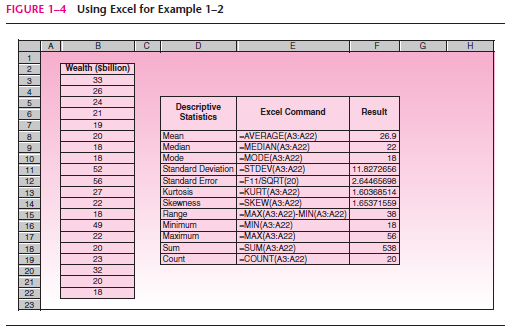
\includegraphics[width=0.5\textwidth]{assets/images/statistics/basic-statistics/excel-formulae.png} 

\clearpage

\subsection*{Skewness } 

is a way to describe the symmetry of a distribution.

A distribution is \textbf{left skewed} if it has a “tail” on the left side of the distribution: 

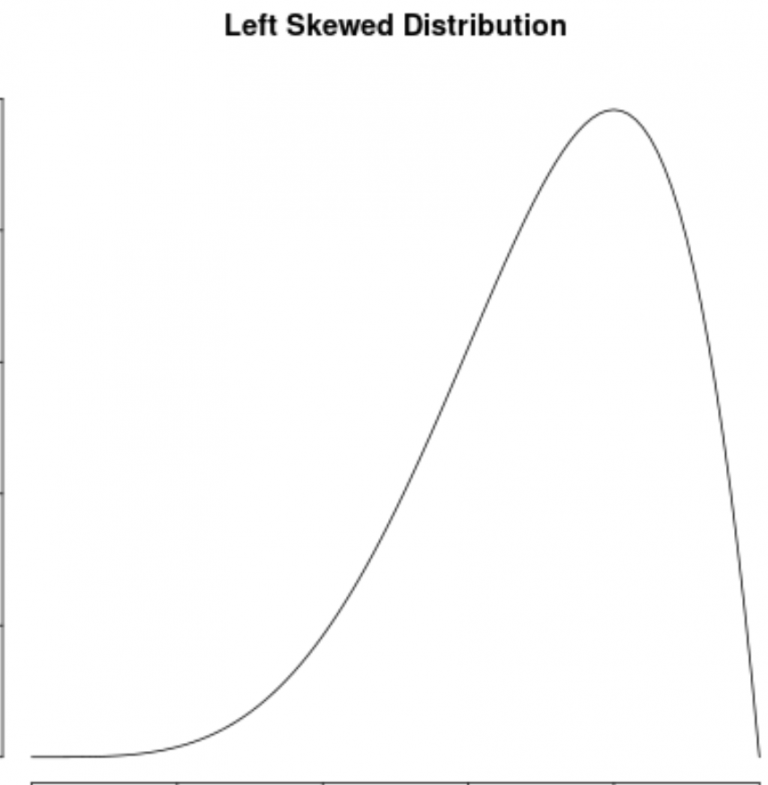
\includegraphics[width=0.5\textwidth]{assets/images/statistics/basic-statistics/left-skew.png} 
    
A distribution is \textbf{right skewed} if it has a “tail” on the right side of the distribution:

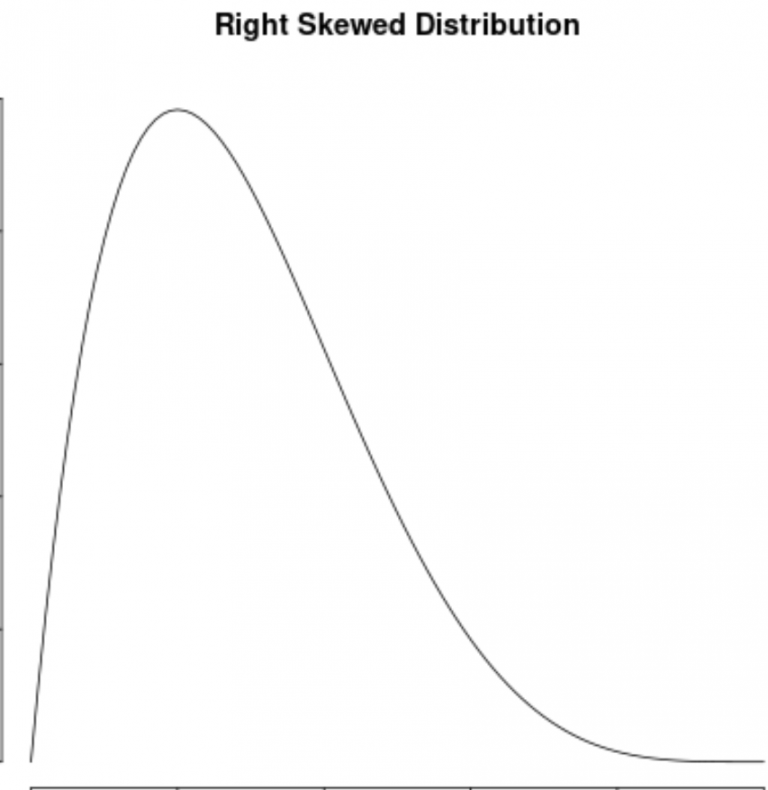
\includegraphics[width=0.5\textwidth]{assets/images/statistics/basic-statistics/right-skew.png}






\subsection*{Properties of Skewed Distributions }

The following diagrams show where the mean, median and mode are typically located in different distributions.

\textbf {Left Skewed Distribution}: \(Mean < Median < Mode\)

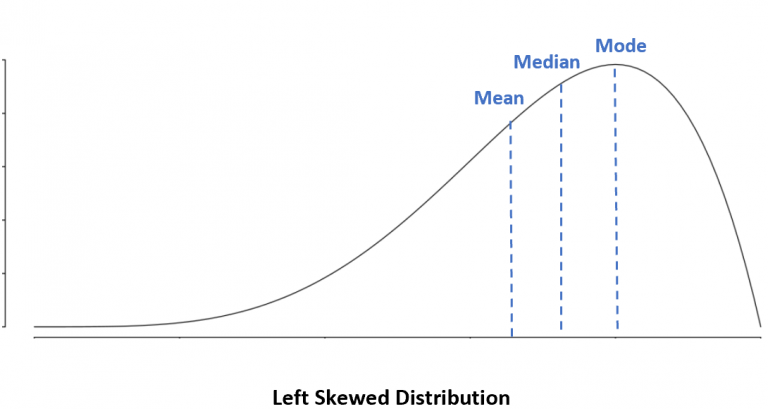
\includegraphics[width=0.5\textwidth]{assets/images/statistics/basic-statistics/left-skew-distribution.png}

\textbf{Right Skewed Distribution}: Mode < Median < Mean

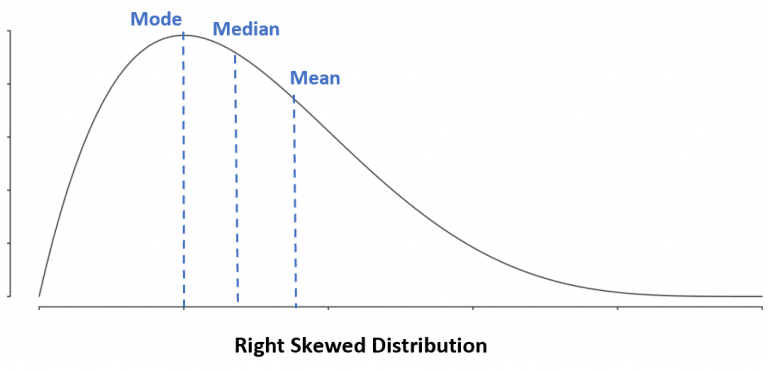
\includegraphics[width=0.5\textwidth]{assets/images/statistics/basic-statistics/right-skew-distribution.png}

\subsection*{Using Box Plots to Visualize Skewness}

A box plot is a type of plot that displays the five number summary of a dataset, which includes:
\begin{itemize}
    \item The minimum value
    \item The first quartile (the 25th percentile)
    \item The median value
    \item The third quartile (the 75th percentile)
    \item The maximum value
\end{itemize}
  
To make a box plot, we draw a box from the first to the third quartile. Then we draw a vertical line at the median. Lastly, we draw “whiskers” from the quartiles to the minimum and maximum value.

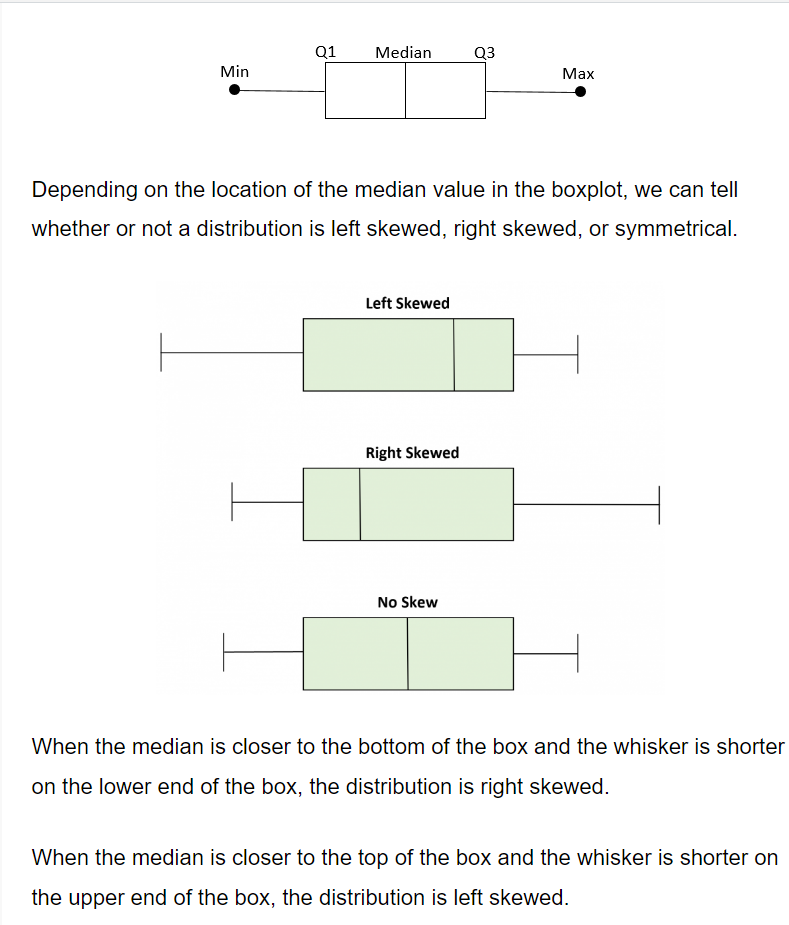
\includegraphics[width=0.5\textwidth]{assets/images/statistics/basic-statistics/skewness-with-box-plot.png} % Replace with your image file


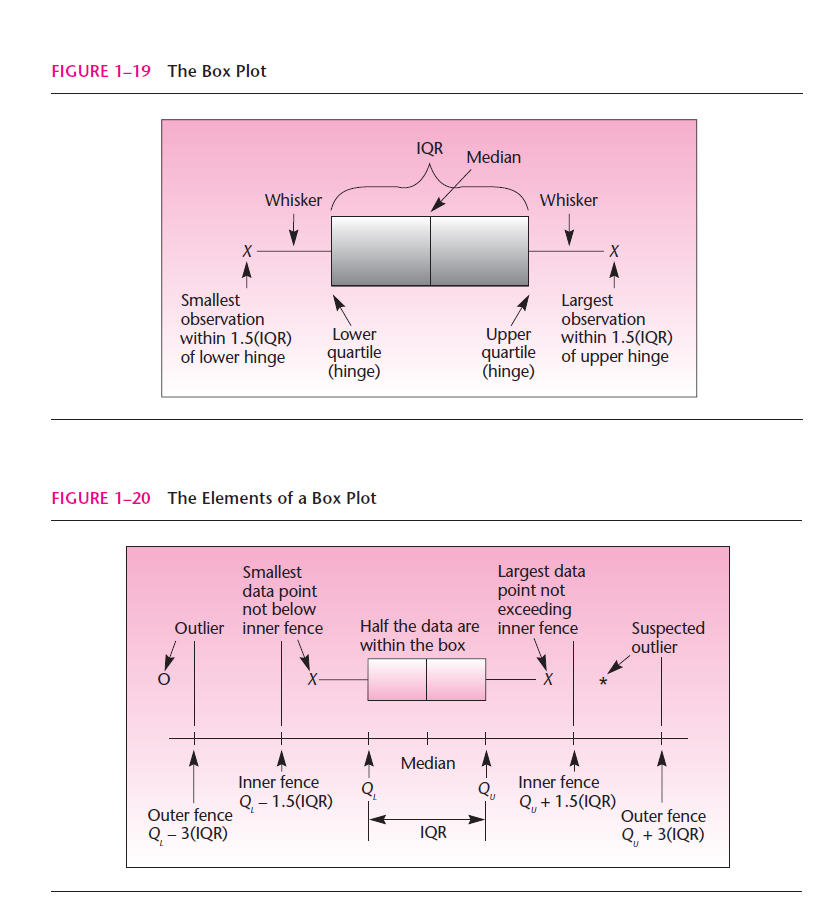
\includegraphics[width=0.5\textwidth]{assets/images/statistics/basic-statistics/whishker-plot-details.png} % Replace with your image file

\clearpage
\section{DESCRIPTIVE AND INFERENTIAL
STATISTICS}\label{descriptive-and-inferential-statistics}

\subsubsection{\texorpdfstring{\textbf{Descriptive and Inferential
Statistics:}}{Descriptive and Inferential Statistics:}}\label{descriptive-and-inferential-statistics-1}

In statistics, \textbf{descriptive} and \textbf{inferential statistics}
are two key branches that help us make sense of data. Each has a
distinct purpose and set of methods.

\begin{center}\rule{0.5\linewidth}{0.5pt}\end{center}

\subsubsection{\texorpdfstring{\textbf{1. Descriptive
Statistics:}}{1. Descriptive Statistics:}}\label{descriptive-statistics}

\textbf{Purpose:} Descriptive statistics aim to summarize, organize, and
simplify large amounts of data into manageable forms that give insights
about the data without drawing conclusions beyond the dataset itself.

\begin{itemize}
\tightlist
\item
  \textbf{Used for:} Providing a clear snapshot of the data.
\item
  \textbf{Focus:} Describing the characteristics of the dataset.
\end{itemize}

\paragraph{\texorpdfstring{\textbf{Key Components of Descriptive
Statistics:}}{Key Components of Descriptive Statistics:}}\label{key-components-of-descriptive-statistics}

\begin{enumerate}
\def\labelenumi{\arabic{enumi}.}
\tightlist
\item
  \textbf{Measures of Central Tendency:}

  \begin{itemize}
  \tightlist
  \item
    These describe the center of the data distribution.

    \begin{itemize}
    \tightlist
    \item
      \textbf{Mean:} The average value.
    \item
      \textbf{Median:} The middle value when data is ordered.
    \item
      \textbf{Mode:} The most frequent value.
    \end{itemize}
  \end{itemize}

  \textbf{Example:} If we have the data points: {[}1, 2, 2, 3, 4{]}

  \begin{itemize}
  \tightlist
  \item
    \textbf{Mean:} (1 + 2 + 2 + 3 + 4) / 5 = 2.4
  \item
    \textbf{Median:} 2
  \item
    \textbf{Mode:} 2 (appears most frequently)
  \end{itemize}
\item
  \textbf{Measures of Dispersion:}

  \begin{itemize}
  \tightlist
  \item
    These describe the spread or variability in the data.

    \begin{itemize}
    \tightlist
    \item
      \textbf{Range:} Difference between the maximum and minimum values.
    \item
      \textbf{Variance:} The average of the squared differences from the
      mean.
    \item
      \textbf{Standard Deviation:} The square root of the variance. It
      provides an understanding of how much the data deviate from the
      mean.
    \end{itemize}
  \end{itemize}

  \textbf{Example:} If we have the data points: {[}1, 2, 2, 3, 4{]}

  \begin{itemize}
  \tightlist
  \item
    \textbf{Range:} 4 - 1 = 3
  \item
    \textbf{Variance:} 1.3
  \item
    \textbf{Standard Deviation:} 1.14
  \end{itemize}
\item
  \textbf{Shape of the Data Distribution:}

  \begin{itemize}
  \tightlist
  \item
    \textbf{Skewness:} Measures the asymmetry of the distribution.

    \begin{itemize}
    \tightlist
    \item
      \textbf{Right-skewed (Positive skewness):} Tail is on the right
      side (e.g., income data).
    \item
      \textbf{Left-skewed (Negative skewness):} Tail is on the left
      side.
    \end{itemize}
  \item
    \textbf{Kurtosis:} Measures the ``tailedness'' of the distribution
    (sharp peak vs.~flat peak).
  \end{itemize}
\item
  \textbf{Percentiles and Quartiles:}

  \begin{itemize}
  \tightlist
  \item
    \textbf{Percentiles:} Describe the percentage of data below a
    certain value (e.g., 50th percentile is the median).
  \item
    \textbf{Quartiles:} Divide data into four equal parts:

    \begin{itemize}
    \tightlist
    \item
      \textbf{Q1 (25th percentile):} Lower quartile.
    \item
      \textbf{Q2 (50th percentile):} Median.
    \item
      \textbf{Q3 (75th percentile):} Upper quartile.
    \end{itemize}
  \item
    \textbf{Interquartile Range (IQR):} Q3 - Q1, measures the spread of
    the middle 50\% of the data.
  \end{itemize}
\end{enumerate}

\paragraph{\texorpdfstring{\textbf{Visualization
Tools:}}{Visualization Tools:}}\label{visualization-tools}

\begin{itemize}
\tightlist
\item
  \textbf{Histograms:} Show frequency distribution.
\item
  \textbf{Bar Charts:} Display categorical data.
\item
  \textbf{Box Plots:} Show median, quartiles, and outliers.
\item
  \textbf{Scatter Plots:} Show relationships between two variables.
\end{itemize}

\paragraph{\texorpdfstring{\textbf{Example of Descriptive Statistics in
Action:}}{Example of Descriptive Statistics in Action:}}\label{example-of-descriptive-statistics-in-action}

Suppose you are analyzing the test scores of students in a class: -
\textbf{Mean:} 75 - \textbf{Median:} 78 - \textbf{Standard Deviation:}
10 (shows how spread out the scores are) - \textbf{Skewness:} Slightly
left-skewed (more students scored higher than the mean)

In \textbf{descriptive statistics}, you are simply summarizing the data,
not making any predictions or inferences.

\begin{center}\rule{0.5\linewidth}{0.5pt}\end{center}

\subsubsection{\texorpdfstring{\textbf{2. Inferential
Statistics:}}{2. Inferential Statistics:}}\label{inferential-statistics}

\textbf{Purpose:} Inferential statistics go beyond merely describing the
data. It allows you to make conclusions or \textbf{inferences} about a
population based on a sample of data.

\begin{itemize}
\tightlist
\item
  \textbf{Used for:} Making predictions, estimations, and testing
  hypotheses.
\item
  \textbf{Focus:} Drawing conclusions about a larger population from a
  sample.
\end{itemize}

\paragraph{\texorpdfstring{\textbf{Key Components of Inferential
Statistics:}}{Key Components of Inferential Statistics:}}\label{key-components-of-inferential-statistics}

\begin{enumerate}
\def\labelenumi{\arabic{enumi}.}
\item
  \textbf{Sampling:}

  \begin{itemize}
  \tightlist
  \item
    A sample is a subset of the population. Inferential statistics uses
    samples to make predictions about the population.
  \item
    \textbf{Random sampling} ensures that every member of the population
    has an equal chance of being selected.
  \end{itemize}
\item
  \textbf{Estimation:}

  \begin{itemize}
  \tightlist
  \item
    \textbf{Point Estimation:} Estimating a population parameter (e.g.,
    population mean) using a single value based on sample data.
  \item
    \textbf{Interval Estimation:} Calculating an interval within which
    the population parameter is likely to lie (e.g., confidence
    intervals).
  \end{itemize}

  \textbf{Example:} You may estimate that the average height of a
  population is 170 cm, but you also give a confidence interval of 168
  cm to 172 cm, meaning you are confident the true average lies within
  that range.
\item
  \textbf{Hypothesis Testing:}

  \begin{itemize}
  \tightlist
  \item \textbf{Null Hypothesis \(H_{0}\):} Assumes no effect or no difference.
  \item textbf{Alternative Hypothesis \(H_{1}\):} Assumes there is an effect or
    a difference.
  \item
    A test (e.g., t-test, ANOVA, chi-square) is performed to decide
    whether to reject or fail to reject the null hypothesis.
  \end{itemize}

  \textbf{Key Concepts in Hypothesis Testing:}

  \begin{itemize}
  \tightlist
  \item
    \textbf{P-value:} The probability of observing the test results
    under the null hypothesis. A small p-value (typically less than
    0.05) indicates that you should reject the null hypothesis.
  \item
    \textbf{Type I Error:} Rejecting the null hypothesis when it is
    actually true (false positive).
  \item
    \textbf{Type II Error:} Failing to reject the null hypothesis when
    it is actually false (false negative).
  \end{itemize}
\item
  \textbf{Confidence Intervals:}

  \begin{itemize}
  \tightlist
  \item
    A range of values used to estimate the true value of a population
    parameter. For example, a 95\% confidence interval means that if you
    repeated the experiment many times, the true parameter would lie
    within this interval in 95\% of the cases.
  \end{itemize}

  \textbf{Example:} Estimating the mean height of a population is 170 cm
  with a 95\% confidence interval of {[}168 cm, 172 cm{]}.
\item
  \textbf{Regression Analysis:}

  \begin{itemize}
  \tightlist
  \item
    \textbf{Simple Linear Regression:} Examines the relationship between
    two continuous variables.
  \item
    \textbf{Multiple Linear Regression:} Explores the relationship
    between one dependent variable and multiple independent variables.
  \item
    \textbf{Logistic Regression:} Used for classification tasks (e.g.,
    predicting binary outcomes).
  \end{itemize}

  \textbf{Example:} Predicting house prices based on features like
  square footage, location, and number of bedrooms using linear
  regression.
\end{enumerate}

\paragraph{\texorpdfstring{\textbf{Example of Inferential Statistics in
Action:}}{Example of Inferential Statistics in Action:}}\label{example-of-inferential-statistics-in-action}

Suppose you want to estimate the average salary of data scientists in a
country: - You collect a \textbf{sample} of 500 data scientists'
salaries. - Using \textbf{inferential statistics}, you can estimate the
\textbf{mean salary} of all data scientists and calculate a
\textbf{confidence interval} around this estimate. - You can also
perform a \textbf{hypothesis test} to see if the average salary is
significantly different from another country's average.

\begin{center}\rule{0.5\linewidth}{0.5pt}\end{center}

\clearpage

\subsubsection{\texorpdfstring{\textbf{Key Differences Between
Descriptive and Inferential
Statistics:}}{Key Differences Between Descriptive and Inferential Statistics:}}\label{key-differences-between-descriptive-and-inferential-statistics}

\begin{longtable}[]{@{}
  >{\raggedright\arraybackslash}p{(\linewidth - 4\tabcolsep) * \real{0.1491}}
  >{\raggedright\arraybackslash}p{(\linewidth - 4\tabcolsep) * \real{0.4099}}
  >{\raggedright\arraybackslash}p{(\linewidth - 4\tabcolsep) * \real{0.4410}}@{}}
\toprule\noalign{}
\begin{minipage}[b]{\linewidth}\raggedright
\textbf{Feature}
\end{minipage} & \begin{minipage}[b]{\linewidth}\raggedright
\textbf{Descriptive Statistics}
\end{minipage} & \begin{minipage}[b]{\linewidth}\raggedright
\textbf{Inferential Statistics}
\end{minipage} \\
\midrule\noalign{}
\endhead
\bottomrule\noalign{}
\endlastfoot
\textbf{Purpose} & Summarize and describe data. & Make predictions or
inferences about a population based on a sample. \\
\textbf{Focus} & Describing the characteristics of a dataset. & Drawing
conclusions beyond the dataset. \\
\textbf{Methods Used} & Measures of central tendency, dispersion, and
distribution. & Estimation, hypothesis testing, regression, confidence
intervals. \\
\textbf{Data Scope} & Works with entire dataset (population or sample).
& Works with a sample to infer about the population. \\
\textbf{Typical Output} & Mean, median, mode, variance, standard
deviation, percentiles. & P-values, confidence intervals, regression
coefficients, test results. \\
\textbf{Examples} & Describing average height or test scores in a
sample. & Estimating average height or salary of a population from a
sample. \\
\end{longtable}

\begin{center}\rule{0.5\linewidth}{0.5pt}\end{center}

\subsubsection{\texorpdfstring{\textbf{Components to Prepare for an
Interview:}}{Components to Prepare for an Interview:}}\label{components-to-prepare-for-an-interview}

When preparing for an interview on statistics, here are key concepts and
topics you should be well-versed in:

\paragraph{\texorpdfstring{\textbf{1. Descriptive
Statistics:}}{1. Descriptive Statistics:}}\label{descriptive-statistics-1}

\begin{itemize}
\tightlist
\item
  Understand measures of central tendency (mean, median, mode).
\item
  Know measures of dispersion (variance, standard deviation, range).
\item
  Be familiar with concepts like skewness and kurtosis.
\item
  Understand different types of data (nominal, ordinal, interval,
  ratio).
\item
  Know how to use visualizations like histograms, box plots, and scatter
  plots.
\end{itemize}

\paragraph{\texorpdfstring{\textbf{2. Inferential
Statistics:}}{2. Inferential Statistics:}}\label{inferential-statistics-1}

\begin{itemize}
\tightlist
\item
  \textbf{Sampling Methods:} Random sampling, stratified sampling, etc.
\item
  \textbf{Estimation:} Point estimates and confidence intervals.
\item
  \textbf{Hypothesis Testing:}

  \begin{itemize}
  \tightlist
  \item
    Null and alternative hypotheses.
  \item
    P-value interpretation.
  \item
    Type I and Type II errors.
  \item
    Understanding of common tests like t-test, ANOVA, chi-square test.
  \end{itemize}
\item
  \textbf{Regression Analysis:}

  \begin{itemize}
  \tightlist
  \item
    Simple and multiple linear regression.
  \item
    Assumptions of linear regression.
  \item
    Logistic regression for classification problems.
  \end{itemize}
\item
  \textbf{Correlation vs.~Causation:} Understand the difference and when
  each applies.
\item
  \textbf{Statistical Significance:} What p-values and confidence
  intervals mean in practice.
\end{itemize}

\paragraph{\texorpdfstring{\textbf{3. Key Probability
Concepts:}}{3. Key Probability Concepts:}}\label{key-probability-concepts}

\begin{itemize}
\tightlist
\item
  \textbf{Basic Probability Theory:} Probability rules, conditional
  probability, independence.
\item
  \textbf{Distributions:}

  \begin{itemize}
  \tightlist
  \item
    Normal distribution, t-distribution, chi-square distribution.
  \item
    Understand probability density functions and cumulative distribution
    functions.
  \end{itemize}
\item
  \textbf{Central Limit Theorem:} Know its importance in inferential
  statistics.
\item
  \textbf{Bayesian Statistics:} Familiarity with the concept of updating
  beliefs using Bayes' theorem (optional but beneficial
\end{itemize}

).

\paragraph{\texorpdfstring{\textbf{4. Common
Tools:}}{4. Common Tools:}}\label{common-tools}

\begin{itemize}
\tightlist
\item
  \textbf{Software:} Be comfortable with tools like R, Python (NumPy,
  pandas, SciPy), and Excel for performing statistical analysis.
\item
  \textbf{Libraries for Visualization:} Seaborn, Matplotlib (in Python),
  ggplot (in R).
\end{itemize}

\paragraph{\texorpdfstring{\textbf{5. Practical
Application:}}{5. Practical Application:}}\label{practical-application}

\begin{itemize}
\tightlist
\item
  Be ready to discuss examples from real-world projects where you
  applied descriptive or inferential statistics.
\item
  Prepare to answer questions on how to handle missing data, outliers,
  or imbalanced datasets.
\end{itemize}

\begin{center}\rule{0.5\linewidth}{0.5pt}\end{center}

By mastering these topics, you will be well-prepared for interviews
involving statistics and data analysis.

\subsubsection{\texorpdfstring{\textbf{5.
Skewness:}}{5. Skewness:}}\label{skewness}

\begin{figure}
\centering
\pandocbounded{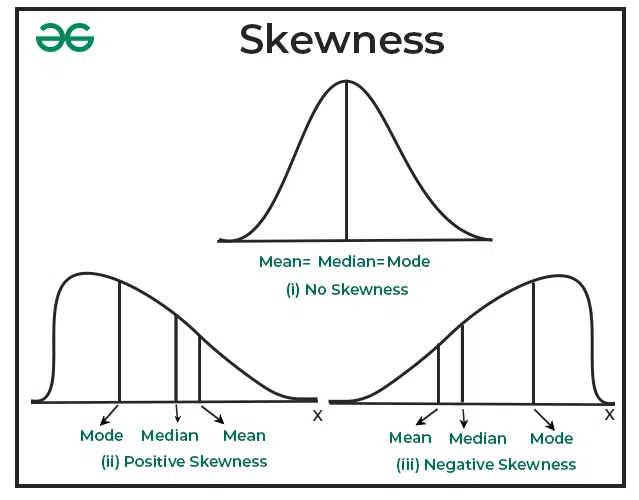
\includegraphics[keepaspectratio]{images/skewness.png}}
\caption{Skewness}
\end{figure}

\subsubsection{Type I and Type II error
Examples}\label{type-i-and-type-ii-error-examples}

In statistics, Type I and Type II errors are concepts related to
hypothesis testing. Here's a brief overview of each along with examples:

\subsubsection{Type I Error (False
Positive)}\label{type-i-error-false-positive}

A Type I error occurs when the null hypothesis is rejected when it is
actually true. In other words, it's the mistake of concluding that there
is an effect or difference when, in reality, there is none.

\textbf{Example 1}: A medical test for a disease - Null Hypothesis (H0):
The patient does not have the disease. - Alternative Hypothesis (H1):
The patient has the disease. - \textbf{Type I Error}: The test indicates
that the patient has the disease when they actually do not (the test
returns a positive result falsely).

\textbf{Example 2}: A new drug's effectiveness - Null Hypothesis (H0):
The new drug has no effect on patients. - Alternative Hypothesis (H1):
The new drug improves patient outcomes. - \textbf{Type I Error}:
Concluding that the new drug is effective when it is not (the trial
shows a statistically significant positive effect when there isn't one).

\subsubsection{Type II Error (False
Negative)}\label{type-ii-error-false-negative}

A Type II error occurs when the null hypothesis is not rejected when it
is actually false. This means failing to detect an effect or difference
when one actually exists.

\textbf{Example 1}: A medical test for a disease - Null Hypothesis (H0):
The patient does not have the disease. - Alternative Hypothesis (H1):
The patient has the disease. - \textbf{Type II Error}: The test
indicates that the patient does not have the disease when they actually
do (the test returns a negative result falsely).

\textbf{Example 2}: A new drug's effectiveness - Null Hypothesis (H0):
The new drug has no effect on patients. - Alternative Hypothesis (H1):
The new drug improves patient outcomes. - \textbf{Type II Error}:
Concluding that the new drug is not effective when it actually is (the
trial fails to show a statistically significant positive effect when
there is one).

\subsubsection{Summary}\label{summary}

\begin{itemize}
\tightlist
\item
  \textbf{Type I Error} (False Positive): Incorrectly rejecting a true
  null hypothesis (e.g., saying a test is positive when it's not).
\item
  \textbf{Type II Error} (False Negative): Failing to reject a false
  null hypothesis (e.g., saying a test is negative when it is actually
  positive).
\end{itemize}

Both types of errors are important to consider in the design and
interpretation of hypothesis tests, as they can have significant
implications in research, healthcare, and more.

\clearpage

\section{Bias and Variance}

\paragraph*{Bias-Variance Tradeoff -}The \textbf{Bias-Variance Tradeoff} is a fundamental concept in machine learning that describes the balance between two sources of error in a model: \textbf{bias} and \textbf{variance}. Understanding this tradeoff helps to choose the right model complexity and improve model performance by reducing both error sources.

\subsubsection*{Key Concepts:}

\begin{enumerate}
    \item \textbf{Bias}
    \begin{itemize}
        \item [-] Bias is the error due to \textbf{oversimplification} of the model.
        \item [-] A model with high bias tends to underfit the data because it makes \textbf{strong assumptions} about the data.
        \item [-] This leads to poor performance on both training and test data.
    \end{itemize}
    \item \textbf{Variance}
    \begin{itemize}
        \item [-] Variance is the error due to the model being \textbf{too sensitive} to small fluctuations in the training data.
        \item [-] A model with high variance tends to overfit the data because it becomes \textbf{too complex}, capturing noise along with the signal.
        \item [-] While it may perform well on training data, it often performs poorly on unseen test data.
    \end{itemize}
    \item \textbf{Noise}
    \begin{itemize}
        \item [-] Noise refers to the random error or irreducible error that cannot be modeled by the algorithm. It is part of the data and can’t be reduced, so the goal is to minimize bias and variance while accepting some level of noise.
    \end{itemize}
\end{enumerate}


\subsubsection*{Understanding the Bias-Variance Tradeoff:}

The \textbf{Bias-Variance Tradeoff} describes the balancing act between:

\begin{itemize}
    \item [-] \textbf{Bias} (how well the model fits the data) and 
    \item [-] \textbf{Variance} (how sensitive the model is to changes in the training data).

\end{itemize}

When you increase the complexity of a model (e.g., by adding more parameters), the \textbf{bias decreases} but the \textbf{variance increases}. Similarly, simplifying the model decreases variance but increases bias.

The goal in machine learning is to find a model that minimizes both bias and variance to achieve the \textbf{lowest possible error} on unseen data.

\subsubsection*{Graphical Representation:}

Imagine a curve where:

\begin{itemize}
    \item [-] On the \textbf{x-axis}, we have model complexity.
    \item [-] On the \textbf{y-axis}, we have error (test error, bias, variance).
    \item [-] \textbf{High Bias Region (Underfitting)}: At the left end of the graph, the model is too simple, resulting in high bias (underfitting). Both training and test errors are high.
    \item [-] \textbf{High Variance Region (Overfitting)}: At the right end, the model is too complex, resulting in high variance (overfitting). Training error is low, but test error is high.
    \item [-] \textbf{Optimal Point}: The sweet spot in the middle is where the tradeoff is balanced, and the model has the lowest possible test error.
\end{itemize}

\subsubsection*{Formula for Error:}
The total \textbf{error} (expected loss) of a model can be expressed as:

\[
\text{Error} = \text{Bias}^2 + \text{Variance} + \text{Irreducible Noise}
\]

\begin{itemize}
    \item [-] \textbf{Bias}: Measures how far the predicted values are from the true values.
    \item [-] \textbf{Variance}: Measures how much the predictions for a given point vary across different training sets.
    \item [-] \textbf{Irreducible Noise}: Represents randomness in the data that no model can explain.
\end{itemize}


\subsubsection*{Examples to Explain:}
\begin{enumerate}
    \item \textbf{High Bias Example (Underfitting)} Imagine trying to fit a \textbf{linear model} to a complex, non-linear dataset (e.g., quadratic data). The model is too simple to capture the underlying pattern, so it will have \textbf{high bias} and will perform poorly on both the training set and test set. This is known as \textbf{underfitting}.
    \begin{itemize}
        \item [-] \textbf{Bias}: High (because the model doesn't capture the complexity of the data).
        \item [-] \textbf{Variance}: Low (because the model does not change much with different training sets).
    \end{itemize}
    \item \textbf{High Variance Example (Overfitting)} Now imagine fitting a \textbf{high-degree polynomial} to the same dataset. The model becomes too complex and fits the training data almost perfectly, even capturing the noise in the data. When this model is applied to unseen test data, it performs poorly because it has \textbf{memorized} the training data rather than generalizing the underlying pattern. This is called \textbf{overfitting}.
    \begin{itemize}
        \item [-] \textbf{Bias}: Low (because the model fits the training data well).
        \item [-] \textbf{Variance}: High (because the model is overly sensitive to changes in the training data).
    \end{itemize}
    \item \textbf{Balanced Model Example:} The goal is to find a \textbf{middle ground}, such as a \textbf{second-degree polynomial} for a quadratic dataset. This model is complex enough to capture the underlying pattern without overfitting the noise. It generalizes well to unseen data and achieves \textbf{low test error}.
    \begin{itemize}
        \item [-] \textbf{Bias}: Moderate (the model captures the main trend without over-simplifying).
        \item [-] \textbf{Variance}: Moderate (the model doesn't change drastically with different training sets).
    \end{itemize}
\end{enumerate}


\subsubsection*{Visual Explanation:}
\begin{itemize}
    \item [-] \textbf{Underfitting (High Bias)}: Imagine a dartboard. A model with high bias will have darts that are far away from the center (true value) but are all clustered together. This means the model is consistently wrong because of its oversimplification.
    \item [-] \textbf{Overfitting (High Variance)}: In contrast, a model with high variance will have darts that are scattered all over the dartboard. Some may hit the center, but others are far away because the model is too sensitive to small changes.
    \item [-] \textbf{Balanced Model}: The ideal model will have darts that are close to the center and well-clustered, meaning the model is both accurate and consistent.
\end{itemize}


\subsubsection*{Bias-Variance Tradeoff in Action:}

\begin{itemize}
    \item [-] \textbf{High Bias}: When the model is too simple, it fails to capture the true relationship in the data, leading to \textbf{underfitting}. Both training and test errors are high.
    \item [-] \textbf{High Variance}: When the model is too complex, it fits the training data too well (including the noise), leading to \textbf{overfitting}. The training error is low, but the test error is high.
    \item [-] \textbf{Optimal Tradeoff}: The best model is the one that balances bias and variance, achieving the lowest error on unseen test data.
\end{itemize}


\subsubsection*{Choosing the Right Model Complexity:}

\begin{itemize}
    \item [-] \textbf{Simpler Models} (e.g., linear regression, shallow decision trees) are prone to high bias and are likely to underfit.
    \item [-] \textbf{Complex Models} (e.g., deep neural networks, high-degree polynomials) are prone to high variance and are likely to overfit.
    \item [-] \textbf{Regularization} techniques like \textbf{Lasso} and \textbf{Ridge Regression} can help reduce variance by penalizing complexity and preventing overfitting.
\end{itemize}


\subsubsection*{Summary:}

\begin{itemize}
    \item [-] \textbf{Bias}: The error due to overly simplistic assumptions. Leads to underfitting.
    \item [-] \textbf{Variance}: The error due to excessive sensitivity to small fluctuations. Leads to overfitting.
    \item [-] The \textbf{Bias-Variance Tradeoff} shows that improving one usually worsens the other. The goal is to find a balance between bias and variance for optimal model performance.
\end{itemize}

\clearpage

\section{\textbf{Standardization vs. Normalization}}

Both standardization and normalization are techniques used in data preprocessing to adjust the scale of the data. These methods are particularly useful in machine learning and statistical modeling.


\subsection*{\textbf{Standardization}}

\begin{itemize}
    \item [-] \textbf{Definition}: It rescales data to have a mean of\textbf{0} and a standard deviation of\textbf{1} (unit variance). 
    \item [-] \textbf{Formula}:
    \[
        z = \frac{x - \mu}{\sigma}
    \]
    where:
    \begin{itemize}
        \item [-] \( x \) is the data point,
        \item [-] \( \mu \) is the mean of the dataset,
        \item [-] \( \sigma \) is the standard deviation of the dataset.
    \end{itemize}
\end{itemize}

\textbf{Use case}: Standardization is often used when the dataset contains features with different units (e.g., age in years and income in dollars) and algorithms like SVMs or logistic regression assume features are normally distributed.

\textbf{Example}:
Suppose we have a dataset with a feature:
\[
[10, 20, 30, 40, 50]
\]
\begin{itemize}
    \item [-] Mean (\( \mu \)) = \( 30 \),
    \item [-] Standard deviation (\( \sigma \)) = \( 14.14 \).
\end{itemize}

Standardized values:
\[
\text{Standardized values} = \left[ \frac{10-30}{14.14}, \frac{20-30}{14.14}, \frac{30-30}{14.14}, \frac{40-30}{14.14}, \frac{50-30}{14.14} \right]
\]

Result:
\[
[-1.41, -0.71, 0, 0.71, 1.41]
\]


\subsection*{\textbf{Normalization}}

\begin{itemize}
    \item [-] \textbf{Definition}: It rescales the data to fit within a specific range, typically\textbf{[0, 1]}. 
    \item [-] \textbf{Formula}:
    \[
    x_{\text{norm}} = \frac{x - x_{\text{min}}}{x_{\text{max}} - x_{\text{min}}}
    \]
    where:
    \begin{itemize}
        \item [-] \( x \) is the data point,
        \item [-] \( x_{\text{min}} \) and \( x_{\text{max}} \) are the minimum and maximum values in the dataset.
    \end{itemize}

\end{itemize}


\textbf{Use case}: Normalization is used when the data needs to be constrained within a fixed range, such as for neural networks or distance-based algorithms like k-NN.

\textbf{Example}:
Using the same dataset:
\[
[10, 20, 30, 40, 50]
\]
\begin{itemize}
    \item [-] Minimum (\( x_{\text{min}} \)) = \( 10 \),
    \item [-] Maximum (\( x_{\text{max}} \)) = \( 50 \).
\end{itemize}


Normalized values:
\[
\text{Normalized values} = \left[ \frac{10-10}{50-10}, \frac{20-10}{50-10}, \frac{30-10}{50-10}, \frac{40-10}{50-10}, \frac{50-10}{50-10} \right]
\]
Result:
\[
[0, 0.25, 0.5, 0.75, 1]
\]



\subsection*{\textbf{Key Differences}}

\begin{tabular}{|p{3cm}|p{4cm}|p{5cm}|}
    \hline
    \textbf{Aspect}              & \textbf{Standardization}                   & \textbf{Normalization}   \\ \hline
    \textbf{Range}               & No fixed range (mean = 0, SD = 1)          & Fixed range, typically [0, 1]          \\ \hline
    \textbf{Effect on outliers}  & Less sensitive to outliers                 & Highly sensitive to outliers           \\ \hline
    \textbf{When to use}         & When features follow Gaussian distribution & When scaling to a specific range is needed \\ \hline
\end{tabular}



\subsection*{\textbf{Summary}}

\begin{itemize}
    \item [-] \textbf{Standardization} focuses on centering data (mean=0, SD=1).
    \item [-] \textbf{Normalization} rescales data to a bounded range, such as [0, 1].
\end{itemize}

\section{Covariance and
correlation}\label{covariance-and-correlation}

Covariance is an indicator of the extent to which 2 random variables are
dependent on each other. A higher number denotes higher dependency.
Correlation is a statistical measure that indicates how strongly two
variables are related. The value of covariance lies in the range of \(-\inf \)
and \(+\inf \)

Covariance indicates the direction of the linear relationship between
variables while correlation measures both the strength and direction of
the linear relationship between two variables. Correlation is a function
of the covariance

\begin{figure}
\centering
\pandocbounded{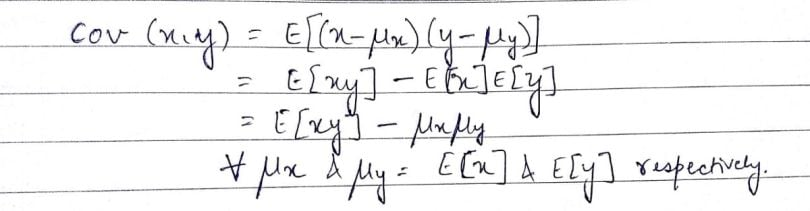
\includegraphics[keepaspectratio]{assets/images/statistics/2022-11-03-07-35-32.png}}
\caption{Covariance}
\end{figure}

\begin{figure}
\centering
\pandocbounded{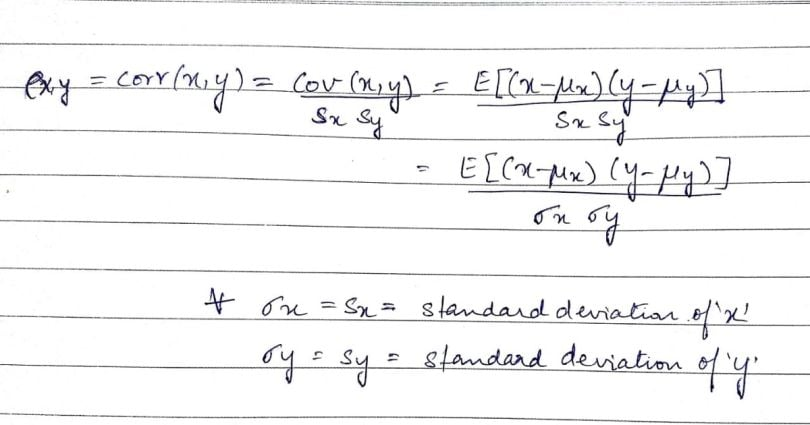
\includegraphics[keepaspectratio]{assets/images/statistics/2022-11-03-07-36-34.png}}
\caption{Correlation}
\end{figure}

\subsubsection{Standard Error and margin of
error}\label{standard-error-and-margin-of-error}

A margin of error is a statistical measure that accounts for the degree
of error received from the outcome of your research sample. On the other
hand, standard error measures the accuracy of the representation of the
population sample to the mean using the standard deviation of the data
set.

How do you find margin of error from standard error? It is calculated
as: \[
\text{Standard Error} = \frac{s}{\sqrt{n}}
\]

\[
\text{Margin of Error} = z \times \frac{s}{\sqrt{n}}
\]

\[
\text{Confidence Interval} = x \pm (z \times \frac{s}{\sqrt{n}})
\]

\subsubsection{Type 1 and Type 2 error}\label{type-1-and-type-2-error}

A type I error (false-positive) occurs if an investigator rejects a null
hypothesis that is actually true in the population; a type II error
(false-negative) occurs if the investigator fails to reject a null
hypothesis that is actually false in the population.

\subsubsection{What is Type 1 and Type 2 error
example?}\label{what-is-type-1-and-type-2-error-example}

Type I error (false positive): the test result says you have
coronavirus, but you actually don't. Type II error (false negative): the
test result says you don't have coronavirus, but you actually do

The \textbf{standard error (SE)} is a statistical term that measures the
accuracy with which a sample distribution represents a population. It
indicates how much variation or ``error'' exists between the sample mean
and the true population mean. Here's a breakdown:

\subsubsection{\texorpdfstring{1.
\textbf{Definition}}{1. Definition}}\label{definition}

The standard error of a statistic (usually the sample mean) is the
\textbf{standard deviation} of the sampling distribution of that
statistic. It quantifies the expected variability of a sample mean (or
other statistic) if you took multiple samples from the same population.

\subsubsection{\texorpdfstring{2.
\textbf{Formula}}{2. Formula}}\label{formula}

For the sample mean, the standard error is calculated as: \[
SE = \frac{\sigma}{\sqrt{n}}
\]

\begin{itemize}
\tightlist
\item
  \(\sigma\): The population standard deviation (if known).
\item
  \textbf{n}: The sample size.
\end{itemize}

If the population standard deviation is not known, it's often estimated
using the sample standard deviation, \((s):\)

\[
SE = \frac{s}{\sqrt{n}}
\]

\subsubsection{\texorpdfstring{3. \textbf{Key
Concepts}}{3. Key Concepts}}\label{key-concepts}

\begin{itemize}
\item
  \textbf{Smaller SE}: A smaller standard error means the sample mean is
  a more precise estimate of the population mean. This happens when the
  sample size (n) is large or the variability (standard deviation, \(\sigma\))
  in the population is small.
\item
  \textbf{Larger SE}: A larger standard error indicates more variability
  in the sample mean, meaning that the sample mean is a less reliable
  estimate of the population mean. This happens when the sample size (n)
  is small or the variability in the population is high.
\end{itemize}

\subsubsection{\texorpdfstring{4. \textbf{Standard Deviation
vs.~Standard
Error}}{4. Standard Deviation vs.~Standard Error}}\label{standard-deviation-vs.-standard-error}

\begin{itemize}
\tightlist
\item
  \textbf{Standard Deviation (SD)} measures the spread of individual
  data points in a population or sample.
\item
  \textbf{Standard Error (SE)} measures the spread of sample means,
  i.e., how much sample means would vary if you repeated your sampling
  multiple times.
\end{itemize}

\subsubsection{\texorpdfstring{5.
\textbf{Importance}}{5. Importance}}\label{importance}

\begin{itemize}
\tightlist
\item
  \textbf{Confidence Intervals}: The SE is used to calculate confidence
  intervals for a sample mean. A smaller SE results in a narrower
  confidence interval, indicating more certainty about the population
  parameter.
\item
  \textbf{Hypothesis Testing}: In many statistical tests (like t-tests),
  SE is used to determine how likely it is that the sample data came
  from a particular population.
\end{itemize}

\subsubsection{Example:}\label{example}

If you take multiple samples from a population and compute the mean of
each sample, the standard error tells you how much the sample means are
likely to differ from the actual population mean. A larger sample size
will decrease the standard error, making your sample mean a more
accurate estimate of the population mean.

\textbf{Normalization} and \textbf{standardization} are techniques used
to adjust data into a consistent format, especially before applying
machine learning models, ensuring different variables are comparable and
models perform optimally. Here's a brief overview of each:

\subsubsection{Normalization}\label{normalization}

Normalization scales data to a specific range, usually between 0 and 1.
It is often used when you want to ensure that all features are on the
same scale, especially when the algorithm you're using is sensitive to
relative magnitudes (e.g., K-nearest neighbors, neural networks).

\textbf{Formula:}

\[
X_{\text{norm}} = \frac{X - X_{\min}}{X_{\max} - X_{\min}}
\]

Where: - \((X)\) is the original data point, - \((X_{\min})\) is the
minimum value of the feature, - \((X_{\max})\) is the maximum value of
the feature.

\subsubsection{When to use
Normalization:}\label{when-to-use-normalization}

\begin{itemize}
\tightlist
\item
  When the features have different ranges but no known normal
  distribution.
\item
  Often for algorithms that calculate distances or require bounded input
  values (like neural networks).
\end{itemize}

\subsubsection{Standardization}\label{standardization}

Standardization (or Z-score normalization) rescales data to have a mean
of 0 and a standard deviation of 1. This is useful when the data is
assumed to have a Gaussian (normal) distribution or when many algorithms
(e.g., linear regression, SVMs) require centered and scaled input.

\textbf{Formula:}

\[
X_{\text{std}} = \frac{X - \mu}{\sigma}
\]

Where: - \((X)\) is the original data point, - \((\mu)\) is the mean of
the feature, - \((\sigma)\) is the standard deviation of the feature.

\subsubsection{When to use
Standardization:}\label{when-to-use-standardization}

\begin{itemize}
\tightlist
\item
  When data follows a normal distribution or can be assumed to.
\item
  When working with algorithms like logistic regression, linear
  regression, or SVM that rely on normally distributed data for optimal
  performance.
\end{itemize}

\subsubsection{Summary:}\label{summary}

\begin{itemize}
\tightlist
\item
  \textbf{Normalization}: Scales values to a range {[}0, 1{]}, often
  used in distance-based algorithms.
\item
  \textbf{Standardization}: Transforms data to have a mean of 0 and a
  standard deviation of 1, suitable for normally distributed data.
\end{itemize}

The choice between normalization and standardization depends on the
model and the nature of the data.


\chapter{Linear Regression}

\section{Interpretation of linear regression}

If all the co-efficent of X is zero in linear regression

\paragraph*{Intercept}{If X sometimes equals 0, the intercept is simply the expected mean value of Y at that value.}


\subsubsection*{The Definition of the Constant is Correct but Misleading}

The constant is often defined as the mean of the dependent variable when you set all of the independent variables in your model to zero. In a purely mathematical sense, this definition is correct. Unfortunately, it’s frequently impossible to set all variables to zero because this combination can be an impossible or irrational arrangement.

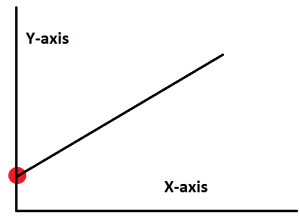
\includegraphics[width=0.5\textwidth]{assets/images/statistics/linear-regression/2022-11-21-08-38-31.png}



\paragraph*{}A portion of the estimation process for the y-intercept is based on the exclusion of relevant variables from the regression model. When you leave relevant variables out, this can produce bias in the model. Bias exists if the residuals have an overall positive or negative mean. In other words, the model tends to make predictions that are systematically too high or too low. The constant term prevents this overall bias by forcing the residual mean to equal zero.


\paragraph*{}Imagine that you can move the regression line up or down to the point where the residual mean equals zero. For example, if the regression produces residuals with a positive average, just move the line up until the mean equals zero. This process is how the constant ensures that the regression model satisfies the critical assumption that the residual average equals zero. However, this process does not focus on producing a y-intercept that is meaningful for your study area. Instead, it focuses entirely on providing that mean of zero.

\paragraph*{}The constant ensures the residuals don’t have an overall bias, but that might make it meaningless.

\subsubsection*{interpretation of negative intercept in regression model}
Depending on your dependent/outcome variable, a negative value for your \(\text{constant}/\text{intercept}\) should not be a cause for concern. This simply means that the expected value on your dependent variable will be less than 0 when all independent/predictor variables are set to 0.



\subsection{The Seven Classical OLS Assumptions}
Like many statistical analyses, ordinary least squares (OLS) regression has underlying assumptions. When these classical assumptions for linear regression are true, ordinary least squares produces the best estimates. However, if some of these assumptions are not true, you might need to employ remedial measures or use other estimation methods to improve the results.

Many of these assumptions describe properties of the error term. Unfortunately, the error term is a population value that we’ll never know. Instead, we’ll use the next best thing that is available—the residuals. Residuals are the sample estimate of the error for each observation.

\[
\text{Residuals} = \text{Observed value} - \text{The fitted value}
\]

When it comes to checking OLS assumptions, assessing the residuals is crucial!

There are seven classical OLS assumptions for linear regression. The first six are mandatory to produce the best estimates. While the quality of the estimates does not depend on the seventh assumption, analysts often evaluate it for other important reasons that I’ll cover.

\subsubsection{OLS Assumption 1: The regression model is linear in the coefficients and the error term}
This assumption addresses the functional form of the model. In statistics, a regression model is linear when all terms in the model are either the constant or a parameter multiplied by an independent variable. You build the model equation only by adding the terms together. These rules constrain the model to one type:

\[
Y =\beta _{0} + \beta _{1}X_{1} + \beta _{2}X_{2} + \cdots + \beta _{k}X_{k} + \epsilon
\]

In the equation, the betas \(\beta s\) are the parameters that OLS estimates. Epsilon \(\epsilon\) is the random error.

In fact, the defining characteristic of linear regression is this functional form of the parameters rather than the ability to model curvature. Linear models can model curvature by including nonlinear variables such as polynomials and transforming exponential functions.

To satisfy this assumption, the correctly specified model must fit the linear pattern.

Related posts: The Difference Between Linear and Nonlinear Regression and How to Specify a Regression Model

\subsubsection{OLS Assumption 2: The error term has a population mean of zero}
The error term accounts for the variation in the dependent variable that the independent variables do not explain. Random chance should determine the values of the error term. For your model to be unbiased, the average value of the error term must equal zero.

Suppose the average error is +7. This non-zero average error indicates that our model systematically underpredicts the observed values. Statisticians refer to systematic error like this as bias, and it signifies that our model is inadequate because it is not correct on average.

Stated another way, we want the expected value of the error to equal zero. If the expected value is +7 rather than zero, part of the error term is predictable, and we should add that information to the regression model itself. We want only random error left for the error term.

You don’t need to worry about this assumption when you include the constant in your regression model because it forces the mean of the residuals to equal zero. For more information about this assumption, read my post about the regression constant.

\subsubsection{OLS Assumption 3: All independent variables are uncorrelated with the error term}
If an independent variable is correlated with the error term, we can use the independent variable to predict the error term, which violates the notion that the error term represents unpredictable random error. We need to find a way to incorporate that information into the regression model itself.

This assumption is also referred to as exogeneity. When this type of correlation exists, there is endogeneity. Violations of this assumption can occur because there is simultaneity between the independent and dependent variables, omitted variable bias, or measurement error in the independent variables.

Violating this assumption biases the coefficient estimate. To understand why this bias occurs, keep in mind that the error term always explains some of the variability in the dependent variable. However, when an independent variable correlates with the error term, OLS incorrectly attributes some of the variance that the error term actually explains to the independent variable instead. For more information about violating this assumption, read my post about confounding variables and omitted variable bias.

Related post: What are Independent and Dependent Variables?

\subsubsection{OLS Assumption 4: Observations of the error term are uncorrelated with each other}
One observation of the error term should not predict the next observation. For instance, if the error for one observation is positive and that systematically increases the probability that the following error is positive, that is a positive correlation. If the subsequent error is more likely to have the opposite sign, that is a negative correlation. This problem is known both as serial correlation and autocorrelation. Serial correlation is most likely to occur in time series models.

For example, if sales are unexpectedly high on one day, then they are likely to be higher than average on the next day. This type of correlation isn’t an unreasonable expectation for some subject areas, such as inflation rates, GDP, unemployment, and so on.

Assess this assumption by graphing the residuals in the order that the data were collected. You want to see randomness in the plot. In the graph for a sales model, there is a cyclical pattern with a positive correlation.

Residuals versus order plot to check the OLS assumption for no serial correlation.
As I’ve explained, if you have information that allows you to predict the error term for an observation, you must incorporate that information into the model itself. To resolve this issue, you might need to add an independent variable to the model that captures this information. Analysts commonly use distributed lag models, which use both current values of the dependent variable and past values of independent variables.

For the sales model above, we need to add variables that explains the cyclical pattern.

Serial correlation reduces the precision of OLS estimates. Analysts can also use time series analysis for time dependent effects.

An alternative method for identifying autocorrelation in the residuals is to assess the autocorrelation function, which is a standard tool in time series analysis.

Related post: Introduction to Time Series Analysis

\subsubsection{OLS Assumption 5: The error term has a constant variance (no heteroscedasticity)}
The variance of the errors should be consistent for all observations. In other words, the variance does not change for each observation or for a range of observations. This preferred condition is known as homoscedasticity (same scatter). If the variance changes, we refer to that as heteroscedasticity (different scatter).

The easiest way to check this assumption is to create a residuals versus fitted value plot. On this type of graph, heteroscedasticity appears as a cone shape where the spread of the residuals increases in one direction. In the graph below, the spread of the residuals increases as the fitted value increases.

Residuals by fitted values plot that displays heteroscedasticity, which violates an OLS assumption.
Heteroscedasticity reduces the precision of the estimates in OLS linear regression.

Related post: Heteroscedasticity in Regression Analysis

Note: When assumption 4 (no autocorrelation) and 5 (homoscedasticity) are both true, statisticians say that the error term is independent and identically distributed (IID) and refer to them as spherical errors.

\subsubsection{OLS Assumption 6: No independent variable is a perfect linear function of other explanatory variables}
Perfect correlation occurs when two variables have a Pearson’s correlation coefficient of +1 or -1. When one of the variables changes, the other variable also changes by a completely fixed proportion. The two variables move in unison.

Perfect correlation suggests that two variables are different forms of the same variable. For example, games won and games lost have a perfect negative correlation (-1). The temperature in Fahrenheit and Celsius have a perfect positive correlation (+1).

Ordinary least squares cannot distinguish one variable from the other when they are perfectly correlated. If you specify a model that contains independent variables with perfect correlation, your statistical software can’t fit the model, and it will display an error message. You must remove one of the variables from the model to proceed.

Perfect correlation is a show stopper. However, your statistical software can fit OLS regression models with imperfect but strong relationships between the independent variables. If these correlations are high enough, they can cause problems. Statisticians refer to this condition as multicollinearity, and it reduces the precision of the estimates in OLS linear regression.

Related post: Multicollinearity in Regression Analysis: Problems, Detection, and Solutions

\subsubsection{OLS Assumption 7: The error term is normally distributed (optional)}
OLS does not require that the error term follows a normal distribution to produce unbiased estimates with the minimum variance. However, satisfying this assumption allows you to perform statistical hypothesis testing and generate reliable confidence intervals and prediction intervals.

The easiest way to determine whether the residuals follow a normal distribution is to assess a normal probability plot. If the residuals follow the straight line on this type of graph, they are normally distributed. They look good on the plot below!

Normal probability plot to assess whether the residuals follow a normal distribution and satisfy the OLS assumption.
If you need to obtain p-values for the coefficient estimates and the overall test of significance, check this assumption!


\subsubsection{PROPERTIES OF LEAST SQUARES}

\begin{enumerate}
    \item Mean of estimated residuals = 0, \( \sum \frac {\hat \epsilon}{n} = 0 \)
    \item Sum of squared residuals is minimized.
    \item Sample correlation between x and \(\hat \epsilon\) is zero (i.e., x and \(\hat \epsilon\) are uncorrelated) \(r\{x, \hat \epsilon\} = 0\)
    \item Sample correlation between \(\hat y\) and \(\hat \epsilon \) is zero
    \item Regression line always goes through the mean of x and y, i.e., the regression line goes through point \((\bar x, \bar y)\)
\end{enumerate}


 \textbf{AIC (Akaike Information Criterion), BIC (Bayesian Information Criterion), and AICc (Corrected AIC)} are statistical tools used to compare models and select the one that best explains the data while penalizing for model complexity to avoid overfitting. Here’s a detailed mathematical explanation:

\begin{enumerate}
    \item \textbf{Akaike Information Criterion (AIC)} - AIC estimates the quality of a model by balancing goodness-of-fit with model complexity.
    \textbf{Formula for AIC:} - 
    \[
    \text{AIC} = -2 \ln(\hat{L}) + 2k
    \]

    Where:
    \begin{itemize}
        \item [-] \(( \hat{L} )\): Maximum likelihood of the model (fit to the data).
        \item [-] \(( k )\): Number of parameters in the model (including intercept).
        \item [-] \(( -2 \ln(\hat{L}) )\): Deviance or negative log-likelihood of the model.
    \end{itemize}
    \textbf{Interpretation:}
    \begin{itemize}
        \item [-] The first term (\( -2 \ln(\hat{L}) \)) rewards goodness-of-fit (lower values indicate better fit).
        \item [-] The second term (\( 2k \)) penalizes for the number of parameters to discourage overfitting.
    \end{itemize}
    \item \textbf{Bayesian Information Criterion (BIC)}
    BIC is similar to AIC but introduces a stronger penalty for model complexity, especially for larger datasets.

    \textbf{Formula for BIC:}
    \[
        \text{BIC} = -2 \ln(\hat{L}) + k \ln(n)
    \]
    Where:
    \begin{itemize}
        \item [-] \(( n )\): Number of data points (sample size).
        \item [-] Other terms (\(( \hat{L} )\), \(( k )\)) are as defined for AIC.
    \end{itemize}
    \textbf{Interpretation:}
    \begin{itemize}
        \item [-] The penalty term (\( k \ln(n) \)) increases with sample size, making BIC more conservative than AIC for large datasets.
        \item [-] Prefer models with lower BIC values.
    \end{itemize}

    \item \textbf{Corrected Akaike Information Criterion (AICc)}
    AICc is a corrected version of AIC designed for small sample sizes, where AIC may overfit. \\
    \textbf{Formula for AICc:} - 
    \[
    \text{AICc} = \text{AIC} + \frac{2k(k+1)}{n - k - 1}
    \]
    Where:
    \begin{itemize}
        \item [-] \(( n )\): Number of data points.
        \item [-] \(( k )\): Number of parameters in the model.
        \item [-] Other terms are as defined for AIC.
    \end{itemize}

    \textbf{Interpretation} -
    \begin{itemize}
        \item [-] The correction term (\( \frac{2k(k+1)}{n - k - 1} \)) increases the penalty when \( n \) is small relative to \( k \).
        \item [-] As \( n \to \infty \), AICc converges to AIC.
    \end{itemize}

    \item Model Selection Criteria
    \begin{itemize}
        \item [-] \textbf{AIC}: Prefer smaller AIC values. Use for general-purpose model selection.
        \item [-] \textbf{BIC}: Prefer smaller BIC values. Use when you want a stronger penalty for complexity.
        \item [-] \textbf{AICc}: Prefer smaller AICc values. Use for small sample sizes (\( n/k < 40 \)).
    \end{itemize}

    \item  Log-Likelihood and Deviance
    To calculate (\( \ln(\hat{L}) )\):
    \[
    \ln(\hat{L}) = -\frac{n}{2} \ln(2\pi\sigma^2) - \frac{\text{RSS}}{2\sigma^2}
    \]
    Where:
    \begin{itemize}
        \item [-] \(( \sigma^2 )\): Variance of residuals.
        \item [-] \(( \text{RSS} )\): Residual Sum of Squares.
    \end{itemize}

    \item Comparison of Criteria
    \begin{itemize}
        \item [-] AIC and AICc focus on prediction accuracy and trade off \\ goodness-of-fit and complexity.
        \item [-] BIC adds a stronger penalty for complexity, favoring simpler models as \(( n )\) increases.
        \item [-] \textbf{Relationship:}
        \[
          \text{AICc} > \text{AIC}, \quad \text{BIC} > \text{AIC} \text{ (for large \( n \))}.
        \]
    \end{itemize}

    \item Practical Example
    For \(( k = 3 ), ( n = 100 ), and ( \hat{L} = 0.8 )\):
    \begin{enumerate}
        \item \(( \ln(\hat{L}) = \ln(0.8) = -0.223 )\).
        \item Calculate:
        \begin{itemize}
            \item  [-] \(( \text{AIC} = -2(-0.223) + 2(3) = 6.446 )\).
            \item [-] \(( \text{BIC} = -2(-0.223) + 3\ln(100) = 14.006 )\).
            \item [-] \(( \text{AICc} = 6.446 + \frac{2(3)(3+1)}{100 - 3 - 1} = 6.698 )\).
        \end{itemize}
    \end{enumerate}
\end{enumerate}

\textbf{Key Points}
\begin{itemize}
    \item [-] Lower AIC, BIC, or AICc indicates a better model.
    \item [-] Use \textbf{AIC} for prediction-oriented tasks, \textbf{BIC} for model parsimony, and \textbf{AICc} for small datasets.
\end{itemize}

\paragraph*{Parsimony - } A parsimonious model aims to explain the data with the minimum number of variables or parameters necessary, avoiding unnecessary complexity.

\section{Understanding R-squared: In depth}

\subsection*{ \textbf{Simplified Definition of R-squared}}

R-squared, or the \textbf{coefficient of determination}, is a statistical measure that tells us how well a regression model explains the variability of the dependent variable (target) using the independent variables (features). 

\begin{itemize}
    \item [-] It answers the question: \textbf{"How much of the variation in the target variable can be explained by the model?"}
    \item [-] R-squared values range from \textbf{0 to 1}:
    \begin{enumerate}
        \item The model explains none of the variation in the target variable.
        \item The model perfectly explains all the variation in the target variable.
    \end{enumerate}
      
\end{itemize}


\subsection*{ \textbf{Mathematical Explanation}}

The formula for R-squared is:
\[
R^2 = 1 - \frac{\text{SS}_{\text{res}}}{\text{SS}_{\text{tot}}}
\]

Where:

\begin{enumerate}
    \item \(\text{SS}_{\text{res}}\) (\textbf{Residual Sum of Squares}): The total squared difference between the actual values (\(y_i\)) and the predicted values (\(\hat{y}_i\)):
            \[
            \text{SS}_{\text{res}} = \sum_{i=1}^n (y_i - \hat{y}_i)^2
            \]
   \item \(\text{SS}_{\text{tot}}\) (\textbf{Total Sum of Squares}): The total squared difference between the actual values (\(y_i\)) and their mean (\(\bar{y}\)):
        \[
        \text{SS}_{\text{tot}} = \sum_{i=1}^n (y_i - \bar{y})^2
        \]
\end{enumerate}

\subsection*{ \textbf{Interpretation}}

\begin{itemize}
    \item [-] \(R^2 = 1\): All predictions are perfect (\(\text{SS}_{\text{res}} = 0\)).
    \item [-] \(R^2 = 0\): The model is as good as simply predicting the mean of \(y\) (\(\text{SS}_{\text{res}} = \text{SS}_{\text{tot}}\)).
    \item [-] \(R^2 < 0\): The model performs worse than predicting the mean, indicating a poor fit.
\end{itemize}

\subsection*{ \textbf{Simplified Example}}

Suppose you're predicting house prices:
1. If \(R^2 = 0.85\), this means \textbf{85\% of the variability in house prices is explained by your model}. 
2. The remaining 15\% is due to other factors not captured by the model or random noise.


\subsection*{ \textbf{How to Explain to Others Easily}}
\(R^2\) is like a report card for your regression model. It tells you how much of the 'story' your model captures about the target variable. If it's close to 1, the model is great. If it's closer to 0, the model isn't doing a good job. Think of it as the percentage of information your model explains.

Would you like a visual example or a Python code snippet to compute R-squared?


\chapter{Cross Entropy}

\section{Cross-Entropy: Theoretical and Mathematical Explanation}

\textbf{Cross-entropy} is a loss function commonly used for classification problems, particularly in neural networks and logistic regression. It measures the difference between two probability distributions—the true distribution and the predicted distribution.

Cross-entropy tells us how well the model's predicted probabilities match the actual labels. If the predicted probabilities are far from the actual labels, the cross-entropy loss will be large. If they are close, the loss will be small.

\section{Theoretical Explanation}

In classification problems, the model predicts the probability that an input belongs to each class. Cross-entropy measures the "distance" between the true label distribution (which is typically one-hot encoded) and the predicted probability distribution.

\subsection{Why Use Cross-Entropy?}
    \begin{itemize}
        \item [-] \textbf{Intuition:} In classification, we want our model to assign high probability to the correct class and low probabilities to incorrect ones. Cross-entropy is designed to penalize incorrect predictions more severely when the model is confident about the wrong class (i.e., when the predicted probability is high for the wrong class).
        \item [-] \textbf{Probability-Based:} Cross-entropy loss is based on the log of the predicted probabilities, meaning that a small difference between predicted and actual probabilities leads to a small loss, while a large difference leads to a large loss.
    \end{itemize}

\section{Mathematical Definition}

For a classification problem with two distributions, say \( P \) (the true label distribution) and \( Q \) (the predicted probability distribution), the cross-entropy between them is defined as:

\[
H(P, Q) = - \sum_{i} P(i) \log Q(i)
\]

Where:
- \( P(i) \) is the true probability of class \( i \),
- \( Q(i) \) is the predicted probability of class \( i \),
- \( \log Q(i) \) is the natural logarithm of the predicted probability of class \( i \).

In practice, \( P(i) \) is typically a one-hot encoded vector (i.e., 1 for the correct class and 0 for all other classes).

\subsection*{Binary Cross-Entropy (for Binary Classification)}

For a binary classification problem where the target \( y \in \{0, 1\} \) and the predicted probability for class 1 is \( \hat{y} \), the binary cross-entropy (or log loss) is:

\[
H(y, \hat{y}) = -[y \log(\hat{y}) + (1 - y) \log(1 - \hat{y})]
\]

Where:
- \( y \) is the true label (0 or 1),
- \( \hat{y} \) is the predicted probability for the positive class (class 1),
- \( 1 - \hat{y} \) is the predicted probability for the negative class (class 0).

This formula computes the loss for a single data point. For a dataset with \( n \) data points, the total binary cross-entropy loss is the average over all data points:

\[
H(y, \hat{y}) = -\frac{1}{n} \sum_{i=1}^{n} [y_i \log(\hat{y_i}) + (1 - y_i) \log(1 - \hat{y_i})]
\]

\subsection{Categorical Cross-Entropy (for Multi-Class Classification)}

For multi-class classification, where there are \( C \) classes and \( y \in \{1, 2, \dots, C\} \) is the true label, the categorical cross-entropy loss is:

$$
H(y, \hat{y}) = - \sum_{i=1}^{C} y_i \log(\hat{y}_i)
$$

Where:
- \( y_i \) is the true label for class \( i \) (typically 1 for the correct class and 0 for all others),
- \( \hat{y}_i \) is the predicted probability for class \( i \).

For a dataset of size \( n \), the total cross-entropy loss is:

$$
H(y, \hat{y}) = -\frac{1}{n} \sum_{i=1}^{n} \sum_{j=1}^{C} y_{ij} \log(\hat{y}_{ij})
$$

This equation calculates the sum of cross-entropies for all classes across all data points, where:
- \( y_{ij} \) is 1 if the \( i \)-th data point belongs to class \( j \) and 0 otherwise,
- \( \hat{y}_{ij} \) is the predicted probability that the \( i \)-th data point belongs to class \( j \).

---

\section{Explanation in Simple Terms}

\subsection{For Binary Classification:}
Think of binary cross-entropy as a measure of how well your model is predicting the probability of a single class. If the model predicts a probability close to 1 for the correct class, the cross-entropy loss will be small. But if it predicts a probability close to 0, the loss will be large.

For example:
\begin{itemize}
    \item [-] If the actual label is \( 1 \) and the model predicts \( \hat{y} = 0.9 \), the loss will be small because the prediction is close to the truth.
    \item [-] If the actual label is \( 1 \) and the model predicts \( \hat{y} = 0.1 \), the loss will be large because the prediction is far from the truth.
\end{itemize}

\subsection{For Multi-Class Classification:}
In a multi-class problem, categorical cross-entropy measures how well the model's predicted probability distribution aligns with the true class distribution. If the model assigns high probability to the correct class and low probabilities to the incorrect ones, the loss is small. If the model assigns a high probability to the wrong class, the loss becomes large.

---

\section{Example (Binary Cross-Entropy)}

Let’s say we are doing binary classification, and we have the following predicted probability \( \hat{y} \) and actual label \( y \):

- \( \hat{y} = 0.9 \), \( y = 1 \) (positive class)

The binary cross-entropy loss would be:

\[
H(y, \hat{y}) = - [1 \cdot \log(0.9) + (1 - 1) \cdot \log(1 - 0.9)] = - \log(0.9)
\]

Using \( \log(0.9) \approx -0.105 \), the loss becomes \( 0.105 \).

---

\section{Why Cross-Entropy Works Well for Classification:}

1. **Penalizes Confident Wrong Predictions**:  
   Cross-entropy punishes confident but wrong predictions more harshly than small mistakes. For example, if a model predicts a class with high confidence (say 0.9 probability) but is wrong, the loss will be large. This encourages the model to be more cautious and only assign high probabilities to the correct classes.

2. **Differentiable**:  
   Cross-entropy is differentiable, meaning it can be used in optimization algorithms like gradient descent. This makes it ideal for neural networks, which rely on backpropagation to adjust model weights based on the derivative of the loss function.

3. **Logarithmic Scaling**:  
   Because it uses the logarithm, cross-entropy scales small probability differences into a larger range, making it sensitive to both small and large differences between predicted and true probabilities.

---

\section{Summary of Key Points:}

\begin{itemize}
    \item [-] \textbf{Cross-entropy} measures the difference between the true labels and predicted probabilities, providing a "penalty" for how far the predictions are from the true labels.
    \item [-] \textbf{Binary cross-entropy} is used for two-class classification, while \textbf{categorical cross-entropy} is used for multi-class classification.
    \item [-] Mathematically, cross-entropy involves taking the negative log of the predicted probability for the true class and summing across all classes (or all data points).
    \item [-] Cross-entropy is a popular loss function for \textbf{classification} tasks because it handles probabilities well and provides a meaningful way to quantify prediction errors.
\end{itemize}

This should help you both understand cross-entropy deeply and explain it effectively!

\chapter{Logistic Regression}

\section{Logistic Regression: Detailed
Explanation}\label{logistic-regression-detailed-explanation}

\textbf{Logistic regression} is a statistical method used for binary
classification problems. It predicts the probability of a binary outcome
(e.g., yes/no, true/false, 0/1) based on one or more independent
variables. Unlike linear regression, it models a non-linear relationship
between the dependent and independent variables to constrain predictions
to a range between 0 and 1.

\begin{center}\rule{0.5\linewidth}{0.5pt}\end{center}

\subsubsection{\texorpdfstring{1. \textbf{Key
Concepts}}{1. Key Concepts}}\label{key-concepts}

\begin{itemize}
\tightlist
\item
  \textbf{Dependent Variable (Output)}: Binary (e.g., \(( y = 0 )\) or
  \(( y = 1 )\) ).
\item
  \textbf{Independent Variables (Features)}: Continuous or categorical
  variables used to make predictions.
\item
  \textbf{Goal}: Estimate the probability \(( P(y=1 \mid x) )\) and
  classify based on a threshold (usually 0.5).
\end{itemize}

\begin{center}\rule{0.5\linewidth}{0.5pt}\end{center}

\subsubsection{\texorpdfstring{2. \textbf{Mathematical
Formulation}}{2. Mathematical Formulation}}\label{mathematical-formulation}

\paragraph{\texorpdfstring{2.1 \textbf{Linear Regression
Hypothesis}}{2.1 Linear Regression Hypothesis}}\label{linear-regression-hypothesis}

In linear regression, the hypothesis is: \[
h(x) = \beta_0 + \beta_1 x_1 + \beta_2 x_2 + \dots + \beta_n x_n
\] However, this can yield predictions outside the range \(([0, 1])\),
which is unsuitable for probabilities.

\paragraph{\texorpdfstring{2.2 \textbf{Logistic Regression
Hypothesis}}{2.2 Logistic Regression Hypothesis}}\label{logistic-regression-hypothesis}

To map predictions to a probability range \(([0, 1])\), logistic
regression applies the \textbf{sigmoid function} (or logistic function)
to the linear equation: \[
P(y=1 \mid x) = \sigma(h(x)) = \frac{1}{1 + e^{-z}}, \quad \text{where } z = \beta_0 + \beta_1 x_1 + \dots + \beta_n x_n
\]

\begin{itemize}
\tightlist
\item
  \textbf{Sigmoid Function}: \(( \sigma(z) )\) squashes any real number
  into a probability value between 0 and 1.
\end{itemize}

\[
\sigma(z) =
\begin{cases} 
\approx 1, & \text{if } z \gg 0 \\
\approx 0, & \text{if } z \ll 0
\end{cases}
\]

\begin{center}\rule{0.5\linewidth}{0.5pt}\end{center}

\subsubsection{\texorpdfstring{3. \textbf{Cost
Function}}{3. Cost Function}}\label{cost-function}

Instead of using Mean Squared Error (MSE), logistic regression uses a
\textbf{log-loss (cross-entropy loss)} to evaluate the model. The cost
function for a single data point is: \[
\text{Cost}(h(x), y) = 
\begin{cases} 
- \log(h(x)), & \text{if } y = 1 \\
- \log(1 - h(x)), & \text{if } y = 0
\end{cases}
\]

This can be combined into a single equation: \[
\text{Cost}(h(x), y) = - \big[ y \log(h(x)) + (1-y) \log(1 - h(x)) \big]
\]

For the entire dataset: \[
J(\beta) = \frac{1}{m} \sum_{i=1}^{m} \Big[- y_i \log(h(x_i)) - (1 - y_i) \log(1 - h(x_i))\Big]
\]

\begin{itemize}
\tightlist
\item
  Minimizing this cost function ensures that the predicted probabilities
  closely match the true labels.
\end{itemize}

\begin{center}\rule{0.5\linewidth}{0.5pt}\end{center}

\subsubsection{\texorpdfstring{4.
\textbf{Optimization}}{4. Optimization}}\label{optimization}

To minimize the cost function, \textbf{Gradient Descent} is used: \[
\beta_j \leftarrow \beta_j - \alpha \frac{\partial J(\beta)}{\partial \beta_j}
\] Where: - \(( \alpha )\): Learning rate -
\(( \frac{\partial J(\beta)}{\partial \beta_j} )\): Gradient of the cost
function w.r.t \(( \beta_j )\)

\begin{center}\rule{0.5\linewidth}{0.5pt}\end{center}

\subsubsection{\texorpdfstring{5. \textbf{Why Use Logistic Regression
Instead of Linear
Regression?}}{5. Why Use Logistic Regression Instead of Linear Regression?}}\label{why-use-logistic-regression-instead-of-linear-regression}

\begin{enumerate}
\def\labelenumi{\arabic{enumi}.}
\tightlist
\item
  \textbf{Prediction Range}:

  \begin{itemize}
  \tightlist
  \item
    Linear regression can produce predictions outside \(([0, 1])\).
  \item
    Logistic regression constrains predictions to probabilities in
    \(([0, 1])\).
  \end{itemize}
\item
  \textbf{Interpretability}:

  \begin{itemize}
  \tightlist
  \item
    Logistic regression directly models probabilities, making it easier
    to interpret outcomes.
  \end{itemize}
\item
  \textbf{Appropriate Loss Function}:

  \begin{itemize}
  \tightlist
  \item
    Linear regression minimizes squared errors, which isn't suitable for
    classification problems.
  \item
    Logistic regression uses log-loss, which penalizes incorrect
    classifications more effectively.
  \end{itemize}
\item
  \textbf{Decision Boundary}:

  \begin{itemize}
  \tightlist
  \item
    Logistic regression defines a decision boundary using the sigmoid
    function. For example, if \(( P(y=1 \mid x) > 0.5 )\), classify as
    \(( 1 )\), else classify as \(( 0 )\).
  \end{itemize}
\item
  \textbf{Linear Assumptions}:

  \begin{itemize}
  \tightlist
  \item
    Linear regression assumes a linear relationship between \(( x )\)
    and \(( y )\), which isn't valid for binary outcomes.
  \item
    Logistic regression assumes a linear relationship between \(( x )\)
    and the log-odds of \(( y )\).
  \end{itemize}
\end{enumerate}

\begin{center}\rule{0.5\linewidth}{0.5pt}\end{center}

\subsubsection{\texorpdfstring{6.
\textbf{Example}}{6. Example}}\label{example}

\textbf{Problem}: Predict whether a student passes (\(( y=1 )\)) or
fails (\(( y=0 )\)) based on study hours (\(( x )\)).

\paragraph{Dataset}\label{dataset}

\begin{longtable}[]{@{}ll@{}}
\toprule\noalign{}
Hours Studied (\(( x )\)) & Pass (\(( y )\)) \\
\midrule\noalign{}
\endhead
\bottomrule\noalign{}
\endlastfoot
1 & 0 \\
2 & 0 \\
3 & 0 \\
4 & 1 \\
5 & 1 \\
6 & 1 \\
\end{longtable}

\paragraph{Steps:}\label{steps}

\begin{enumerate}
\def\labelenumi{\arabic{enumi}.}
\item
  \textbf{Hypothesis}: \[
  P(y=1 \mid x) = \frac{1}{1 + e^{-(\beta_0 + \beta_1 x)}}
  \]
\item
  \textbf{Fit Parameters (\(( \beta_0, \beta_1 )\))}: Using optimization
  (e.g., gradient descent), we estimate \(( \beta_0 )\) and
  \(( \beta_1 )\). Assume: \[
  \beta_0 = -3, \, \beta_1 = 1
  \]
\item
  \textbf{Prediction}: For \(( x = 4 )\): \[
  P(y=1 \mid x=4) = \frac{1}{1 + e^{-(-3 + 1 \cdot 4)}} = \frac{1}{1 + e^{-1}} \approx 0.73
  \] Since \(( 0.73 > 0.5 )\), predict \(( y = 1 )\) (pass).
\end{enumerate}

\begin{center}\rule{0.5\linewidth}{0.5pt}\end{center}

\subsubsection{\texorpdfstring{7.
\textbf{Extensions}}{7. Extensions}}\label{extensions}

\begin{itemize}
\tightlist
\item
  \textbf{Multinomial Logistic Regression}: For multi-class
  classification.
\item
  \textbf{Regularization}: Add terms like \(( L_1 )\) (Lasso) or
  \(( L_2 )\) (Ridge) penalties to prevent overfitting.
\end{itemize}

\begin{center}\rule{0.5\linewidth}{0.5pt}\end{center}

Logistic regression remains popular because of its simplicity,
interpretability, and effectiveness in scenarios where linear models are
sufficient for classification tasks.

\section{\texorpdfstring{\textbf{Assumptions of Logistic
Regression}}{Assumptions of Logistic Regression}}\label{assumptions-of-logistic-regression}

Logistic regression is a popular statistical technique used for modeling
binary outcome variables. However, like any other statistical model, it
relies on certain assumptions to ensure the validity and reliability of
the results. Here are the key assumptions of logistic regression:

\begin{enumerate}
\def\labelenumi{\arabic{enumi}.}
\tightlist
\item
  \textbf{Independence of Observations}: Each observation should be
  independent of the others. This means that the outcome of one
  observation should not affect the outcome of another observation.
\item
  \textbf{Linearity in the Log-Odds}: The relationship between the
  log-odds of the outcome and the predictor variables should be linear.
  This assumption can be checked using plots or by including interaction
  terms in the model.
\item
  \textbf{No or Little Multicollinearity}: Multicollinearity occurs when
  two or more predictor variables are highly correlated with each other.
  This can lead to unstable estimates of the regression coefficients and
  inflated standard errors. It's essential to check for
  multicollinearity using techniques such as variance inflation factor
  (VIF) or correlation matrices.
\item
  \textbf{No Significant Outliers}: Outliers can significantly affect
  the model's estimates and predictions. It's crucial to identify and
  handle outliers using techniques such as winsorization or robust
  regression.
\item
  \textbf{Large Enough Sample Size}: Logistic regression requires a
  sufficiently large sample size to produce reliable estimates. A
  general rule of thumb is to have at least 10 events per predictor
  variable.
\item
  \textbf{No or Little Missing Data}: Missing data can lead to biased
  estimates and reduced model performance. It's essential to handle
  missing data using techniques such as imputation or multiple
  imputation.
\item
  \textbf{Correct Model Specification}: The model should be correctly
  specified, including all relevant predictor variables and
  interactions. Omitting important variables or including irrelevant
  ones can lead to biased estimates and poor model performance.
\item
  \textbf{No or Little Non-Linearity}: Logistic regression assumes a
  linear relationship between the log-odds of the outcome and the
  predictor variables. Non-linearity can be handled using techniques
  such as polynomial transformations or generalized additive models.
\end{enumerate}

\subsection{\texorpdfstring{\textbf{Consequences of Violating
Assumptions}}{Consequences of Violating Assumptions}}\label{consequences-of-violating-assumptions}

Violating the assumptions of logistic regression can lead to:

\begin{itemize}
\tightlist
\item
  Biased estimates of the regression coefficients
\item
  Inflated standard errors
\item
  Poor model performance
\item
  Incorrect predictions
\item
  Reduced model interpretability
\end{itemize}

\subsection{\texorpdfstring{\textbf{Diagnosing Assumption
Violations}}{Diagnosing Assumption Violations}}\label{diagnosing-assumption-violations}

To diagnose assumption violations, you can use various techniques such
as:

\begin{itemize}
\tightlist
\item
  Plots (e.g., residual plots, Q-Q plots)
\item
  Statistical tests (e.g., Hosmer-Lemeshow test, likelihood ratio test)
\item
  Model diagnostics (e.g., VIF, condition index)
\item
  Cross-validation
\end{itemize}

\subsection{\texorpdfstring{\textbf{Addressing Assumption
Violations}}{Addressing Assumption Violations}}\label{addressing-assumption-violations}

To address assumption violations, you can use various techniques such
as:

\begin{itemize}
\tightlist
\item
  Data transformation (e.g., log transformation, standardization)
\item
  Model specification changes (e.g., adding interaction terms,
  polynomial transformations)
\item
  Robust regression techniques (e.g., robust logistic regression,
  generalized linear mixed models)
\item
  Model selection techniques (e.g., stepwise regression, backward
  elimination)
\end{itemize}

By understanding and addressing the assumptions of logistic regression,
you can ensure the validity and reliability of your model's results and
make informed decisions based on your analysis.

\chapter{Principal Component Analysis (PCA)}

\section{Principal component
analysis}\label{principal-component-analysis}

Certainly! Principal Component Analysis (PCA) is a powerful statistical
technique used for dimensionality reduction while preserving as much
variance as possible in a dataset. Here's a detailed explanation, broken
down into concepts, mathematical foundation, and a practical example,
which will help you articulate it well in an interview.

\subsubsection{What is PCA?}\label{what-is-pca}

\begin{itemize}
\tightlist
\item
  \textbf{Purpose}: PCA is primarily used to reduce the number of
  variables (dimensions) in a dataset while retaining most of the
  original variability (information). It's especially useful in
  preprocessing data for machine learning tasks when dealing with
  high-dimensional datasets.
\end{itemize}

\subsubsection{Key Concepts}

\begin{enumerate}
\def\labelenumi{\arabic{enumi}.}
\item
  \textbf{Variance}: Variance measures the spread of data points in a
  dataset. PCA aims to find new axes (principal components) that capture
  the most variance in the data.
\item
  \textbf{Dimensionality}: High-dimensional data can be challenging to
  analyze, visualize, or work with in machine learning models. PCA
  reduces dimensionality without losing significant information.
\item
  \textbf{Orthogonal Transformation}: PCA operates by transforming the
  original variables into a new set of uncorrelated variables (the
  principal components), where each component corresponds to a direction
  in the dataset that maximally captures variance.
\end{enumerate}

\subsubsection{Steps in PCA}\label{steps-in-pca}

\begin{enumerate}
\def\labelenumi{\arabic{enumi}.}
\tightlist
\item
  \textbf{Standardize the Data}:

  \begin{itemize}
  \tightlist
  \item
    Scale the data so that it has a mean of 0 and a standard deviation
    of 1. This step is crucial, especially if variables are measured on
    different scales.
  \end{itemize}
\item
  \textbf{Covariance Matrix Calculation}:

  \begin{itemize}
  \tightlist
  \item
    Compute the covariance matrix to understand how the variables of the
    dataset relate to one another.
  \end{itemize}
\item
  \textbf{Eigenvalue and Eigenvector Calculation}:

  \begin{itemize}
  \tightlist
  \item
    Calculate eigenvalues and eigenvectors of the covariance matrix.
    Eigenvectors represent the directions of maximum variance (principal
    components), and eigenvalues represent the magnitude of variance
    captured in those directions.
  \end{itemize}
\item
  \textbf{Sort Eigenvalues and Eigenvectors}:

  \begin{itemize}
  \tightlist
  \item
    Sort the eigenvalues in descending order and arrange the
    corresponding eigenvectors accordingly. This allows us to identify
    which principal components capture the most variance.
  \end{itemize}
\item
  \textbf{Choose Principal Components}:

  \begin{itemize}
  \tightlist
  \item
    Decide how many principal components to keep, based on the
    cumulative explained variance ratio.
  \end{itemize}
\item
  \textbf{Transform the Data}:

  \begin{itemize}
  \tightlist
  \item
    Project the original data onto the selected principal components to
    obtain the reduced-dimensionality representation.
  \end{itemize}
\end{enumerate}

\subsubsection{Example of PCA}\label{example-of-pca}

Let's illustrate PCA with an example involving a 2D dataset. Suppose we
have a dataset with two features: height and weight of individuals.

\paragraph{Step 1: Create Sample Data}\label{step-1-create-sample-data}

\begin{longtable}[]{@{}ll@{}}
\toprule\noalign{}
Height (cm) & Weight (kg) \\
\midrule\noalign{}
\endhead
\bottomrule\noalign{}
\endlastfoot
175 & 70 \\
180 & 80 \\
165 & 60 \\
170 & 65 \\
160 & 55 \\
\end{longtable}

\paragraph{Step 2: Standardize the
Data}\label{step-2-standardize-the-data}

\begin{itemize}
\tightlist
\item
  Standardize this data to have a mean of 0:

  \begin{itemize}
  \tightlist
  \item
    Calculate the mean and standard deviations of height and weight.
    Normalize each feature.
  \end{itemize}
\end{itemize}

\paragraph{Step 3: Covariance Matrix
Calculation}\label{step-3-covariance-matrix-calculation}

\begin{itemize}
\tightlist
\item
  Calculate the covariance matrix for the standardized data. The
  covariance matrix will help us see how height and weight change
  together.
\end{itemize}

For instance, using values:

\[
Cov(X, Y) = \frac{1}{n-1} \sum (X_i - \bar{X})(Y_i - \bar{Y})
\]

Where \((X)\) is height and \((Y)\) is weight.

\paragraph{Step 4: Eigenvalue and Eigenvector
Calculation}\label{step-4-eigenvalue-and-eigenvector-calculation}

\begin{itemize}
\tightlist
\item
  Compute the eigenvalues and eigenvectors of the covariance matrix.
  Let's say the eigenvalues obtained are \((\lambda_{1} = 2.5)\) and
  \((\lambda_{2} = 0.5)\).
\item
  The corresponding eigenvectors would indicate the directions of these
  variances.
\end{itemize}

\paragraph{Step 5: Sort and Choose Principal
Components}\label{step-5-sort-and-choose-principal-components}

\begin{itemize}
\tightlist
\item
  The first principal component will be the eigenvector with \((\lambda_{1})\)
  (largest eigenvalue), and the second can be ignored if we're reducing
  dimensions.
\end{itemize}

\paragraph{Step 6: Transform the Data}\label{step-6-transform-the-data}

\begin{itemize}
\tightlist
\item
  Multiply the standardized data by the selected eigenvector to get the
  principal component coordinates.
\end{itemize}

For instance, if the eigenvector corresponding to \((\lambda_{1})\) is
\(([0.707, 0.707])\), you would project the standardized data onto this
vector to get the new representation in one dimension along this
principal component.

\subsubsection{Conclusion}\label{conclusion}

\begin{itemize}
\tightlist
\item
  PCA helps in data reduction by transforming the original variables
  into new ones that summarize the original data characteristics. The
  distance between data points reflects similarities, aiding in
  visualization and analysis.
\item
  It has applications in various fields including finance,
  bioinformatics, and image processing among others.
\end{itemize}

\subsubsection{Interview Tips}\label{interview-tips}

\begin{itemize}
\tightlist
\item
  \textbf{Be Clear and Concise}: Explain PCA in steps, relating each
  step back to its purpose and importance.
\item
  \textbf{Use Visuals if Possible}: A drawing showing how PCA takes the
  original data and aligns it along principal components can be very
  illustrative.
\item
  \textbf{Discuss Applications}: Mention where PCA is commonly applied,
  as it shows your understanding of its practical utility.
\item
  \textbf{Express Understanding of Limitations}: Acknowledge that PCA
  assumes linear relationships and may lose some information during
  dimensionality reduction.
\end{itemize}

By structuring your explanation in this way, you can clearly convey the
essence, methodology, and applications of PCA during your interview.


\chapter{Encoding Techniques}

\section{Encoding Techniques in Data Science}

\subsubsection{\texorpdfstring{1. \textbf{OneHot
Encoding}}{1. OneHot Encoding}}\label{onehot-encoding}

\textbf{Definition:} OneHot Encoding converts categorical variables into
binary vectors where each category is represented by a separate column
containing 0s and 1s.

\textbf{Use Cases:} - Suitable for nominal categorical variables (no
order or ranking). - Commonly used in classification models requiring
categorical input.

\textbf{Example:} 

\begin{tabular}{|p{3cm}|p{3cm}|p{3cm}|}
  \hline
  \textbf{Red}              & \textbf{Blue}                   & \textbf{Green}   \\ \hline
\end{tabular}

After OneHot Encoding:

\begin{tabular}{|p{3cm}|p{3cm}|p{3cm}|}
  \hline
  \textbf{Color\_Red}              & \textbf{Color\_Blue}                   & \textbf{Color\_Green}   \\ \hline
  1&0&0 \\ \hline
  0&1&0 \\ \hline
  0&0&1 \\ \hline
\end{tabular}


\vspace{5pt}

\textbf{Mathematics:} - No complex formula; maps each category to a
unique vector.

\textbf{Advantages:} - Prevents the model from assuming any ordinal
relationship. - Widely supported in ML libraries.

\textbf{Disadvantages:} - High cardinality features can create excessive
dimensions, leading to increased model complexity.

\begin{center}\rule{0.5\linewidth}{0.5pt}\end{center}

\subsubsection{\texorpdfstring{2. \textbf{Label
Encoding}}{2. Label Encoding}}\label{label-encoding}

\textbf{Definition:} Label Encoding assigns a unique integer value to
each category in the feature.

\textbf{Use Cases:} - Suitable for ordinal categorical variables (where
order matters). - Useful in tree-based models which can interpret
numerical relationships better.

\textbf{Example:} 

\begin{tabular}{|c|c|c|}
  \hline
  \textbf{Small} & \textbf{Medium} & \textbf{Large} \\ \hline
\end{tabular}

After Label Encoding: 

\begin{tabular}{|c|c|c|}
  \hline
  \textbf{0} & \textbf{1} & \textbf{2} \\ \hline
\end{tabular}


\textbf{Mathematics:} - Maps each unique category to an integer value: \(X_{i} = i \)

\textbf{Advantages:} - Efficient for low-cardinality categorical
features.

\textbf{Disadvantages:} - May introduce an unintended ordinal
relationship in non-ordinal data.

\begin{center}\rule{0.5\linewidth}{0.5pt}\end{center}

\subsubsection{\texorpdfstring{3. \textbf{Ordinal
Encoding}}{3. Ordinal Encoding}}\label{ordinal-encoding}

\textbf{Definition:} Ordinal Encoding assigns integer values to
categories based on their ordinal rank.

\textbf{Use Cases:} - Ideal for ordinal data where category order
carries meaning.

\textbf{Example:} 

\begin{tabular}{|c|c|c|c|c|}
  \hline
  \textbf{Education} & \textbf{High School}  & \textbf{Bachelor’s} & \textbf{Master’s} & \textbf{PhD} \\ \hline
\end{tabular}


After Ordinal Encoding: 

\begin{tabular}{|c|c|c|c|c|}
  \hline
  \textbf{Education} & \textbf{1}  & \textbf{2} & \textbf{3} & \textbf{4} \\ \hline
\end{tabular}


\textbf{Mathematics:} - Assigns ranks to categories, often starting from
1: \( X_{i} = i \)

\textbf{Advantages:} - Preserves meaningful ordinal relationships.

\textbf{Disadvantages:} - Misinterpreting non-ordinal data as ordinal
can mislead the model.

\begin{center}\rule{0.5\linewidth}{0.5pt}\end{center}

\subsubsection{\texorpdfstring{4. \textbf{Target
Encoding}}{4. Target Encoding}}\label{target-encoding}

\textbf{Definition:} Target Encoding replaces each category with the
mean of the target variable for that category.

\textbf{Use Cases:} - Effective for high-cardinality categorical
features in regression problems.

\textbf{Example:} 

\begin{tabular}{|c|c|c|c|}
  \hline
  \textbf{City} & \textbf{House Price} \\ \hline
  A & 300,000 \\ \hline
  B & 500,000 \\ \hline
  A & 310,000 \\ \hline
\end{tabular}


After Target Encoding: 

\begin{tabular}{|c|c|c|c|}
  \hline
  \textbf{City} \\ \hline
  305,000 \\ \hline
  500,000 \\ \hline
  305,000 \\ \hline
\end{tabular}




\textbf{Mathematics:} 

\[ 
X_{i} = \frac{\sum_{y \in Y_{i}} y}{|Y_i|} 
\]

\textbf{Advantages:} - Reduces dimensionality in high-cardinality data.

\textbf{Disadvantages:} - Risk of data leakage; requires proper
cross-validation.

\begin{center}\rule{0.5\linewidth}{0.5pt}\end{center}

\subsubsection{\texorpdfstring{5. \textbf{Frequency
Encoding}}{5. Frequency Encoding}}\label{frequency-encoding}

\textbf{Definition:} Frequency Encoding assigns values based on the
frequency of each category in the dataset.

\textbf{Use Cases:} - Effective for handling categorical variables with
many levels.

\textbf{Example:} 

\begin{tabular}{|c|c|c|c|}
  \hline
  \textbf{City} \\ \hline
  A \\ \hline
  B \\ \hline
  A \\ \hline
\end{tabular}

% \textbar{} City \textbar{} \textbar--------\textbar{}
% \textbar{} A \textbar{} \textbar{} B \textbar{} \textbar{} A \textbar{}

After Frequency Encoding: 

\begin{tabular}{|c|c|c|c|}
  \hline
  \textbf{City} \\ \hline
  2 \\ \hline
  1 \\ \hline
  2 \\ \hline
\end{tabular}


\textbf{Mathematics:} \[ X_{i} = \text{Frequency}(X_{i}) \]

\textbf{Advantages:} - Efficient for high-cardinality data. - Preserves
some information about category importance.

\textbf{Disadvantages:} - Does not capture relationships between
categories and the target variable.

\begin{center}\rule{0.5\linewidth}{0.5pt}\end{center}

\subsubsection{\texorpdfstring{6. \textbf{Embedding
Encoding}}{6. Embedding Encoding}}\label{embedding-encoding}

\textbf{Definition:} Embedding Encoding maps categorical variables into
dense vector spaces, often using neural networks.

\textbf{Use Cases:} - Highly effective for NLP tasks, deep learning
models, and large categorical data with complex relationships.

\textbf{Example:} A ``Movie Genre'' feature encoded into a 3D vector:

\begin{verbatim}
Action  -> [0.9, 0.1, 0.4]
Comedy  -> [0.2, 0.8, 0.3]
Drama   -> [0.1, 0.3, 0.9]
\end{verbatim}

\textbf{Mathematics:} - Learned embeddings are trained through
backpropagation in neural networks. - Each category \( X_{i} \) is mapped
to a vector \( v_{i} \) in \( R^{d} \).

\textbf{Advantages:} - Captures rich semantic information. - Efficient
for high-dimensional categorical data.

\textbf{Disadvantages:} - Requires model training, making it
computationally expensive.


\chapter{Decision Tree}

A decision tree is a supervised learning algorithm used for both
classification and regression tasks. It works by splitting the data into
subsets based on the values of the attributes, which helps to make
predictions about the target variable. One of the common metrics used
for determining how to split the data at each node is \textbf{entropy}.
Entropy measures the uncertainty or impurity in a dataset.

\subsubsection{Entropy Calculation}\label{entropy-calculation}

The entropy \(( H )\) of a dataset can be calculated using the formula:

\[
H(S) = -\sum_{i=1}^{c} p_i \log_2(p_i)
\]

where: - \(( S )\) is the dataset. - \(( c )\) is the number of classes.
- \(( p_{i} )\) is the proportion of instances in class \(( i )\).

\subsubsection{Example Scenario}\label{example-scenario}

Let's consider a simple example to demonstrate how a decision tree
works, specifically using entropy to determine the best splits.

\textbf{Dataset:} Assume we have a dataset of 10 instances with the
following attributes:

\begin{longtable}[]{@{}ll@{}}
\toprule\noalign{}
Weather & Play (Target) \\
\midrule\noalign{}
\endhead
\bottomrule\noalign{}
\endlastfoot
Sunny & No \\ \hline
Sunny & No \\ \hline
Overcast & Yes \\ \hline
Rainy & Yes \\ \hline
Rainy & Yes \\ \hline
Rainy & No \\ \hline
Overcast & Yes \\ \hline
Sunny & Yes \\ \hline
Sunny & No \\ \hline
Rainy & Yes \\ \hline
\end{longtable}

The classes for the target variable ``Play'' are \textbf{Yes} and
\textbf{No}.

\paragraph{Step 1: Calculate the Initial
Entropy}\label{step-1-calculate-the-initial-entropy}

\begin{enumerate}
\def\labelenumi{\arabic{enumi}.}
\tightlist
\item
  \textbf{Count the instances}:

  \begin{itemize}
  \tightlist
  \item
    Total instances = 10
  \item
    Instances of ``Yes'' = 5
  \item
    Instances of ``No'' = 5
  \end{itemize}
\item
  \textbf{Calculate the probabilities}:

  \begin{itemize}
  \tightlist
  \item
    \(( p_{\text{Yes}} = \frac{5}{10} = 0.5 )\)
  \item
    \(( p_{\text{No}} = \frac{5}{10} = 0.5 )\)
  \end{itemize}
\item
  \textbf{Calculate the entropy}: \[
  H(S) = -\left(0.5 \log_2(0.5) + 0.5 \log_2(0.5)\right) = -\left(0.5 \cdot (-1) + 0.5 \cdot (-1)\right) = 1
  \]
\end{enumerate}

So the initial entropy \(( H(S) = 1 )\).

\paragraph{Step 2: Calculate Entropy for Each
Split}\label{step-2-calculate-entropy-for-each-split}

Let's consider splitting on the ``Weather'' attribute.

\begin{enumerate}
\def\labelenumi{\arabic{enumi}.}
\tightlist
\item
  \textbf{Weather = Sunny}:

  \begin{itemize}
  \tightlist
  \item
    Instances: 3 (2 No, 1 Yes)
  \item
    Probabilities:

    \begin{itemize}
    \tightlist
    \item
      \(( p_{\text{Yes}} = \frac{1}{3} )\)
    \item
      \(( p_{\text{No}} = \frac{2}{3} )\)
    \end{itemize}
  \item
    Entropy: \[
    H(\text{Sunny}) = -\left(\frac{1}{3} \log_2\left(\frac{1}{3}\right) + \frac{2}{3} \log_2\left(\frac{2}{3}\right)\right) \approx -\left(\frac{1}{3} \cdot (-1.585) + \frac{2}{3} \cdot (-0.585)\right) \approx 0.918
    \]
  \end{itemize}
\item
  \textbf{Weather = Overcast}:

  \begin{itemize}
  \tightlist
  \item
    Instances: 2 (Both Yes)
  \item
    Probabilities:

    \begin{itemize}
    \tightlist
    \item
      \(( p_{\text{Yes}} = 1 )\)
    \item
      \(( p_{\text{No}} = 0 )\)
    \end{itemize}
  \item
    Entropy: \[
    H(\text{Overcast}) = -\left(1 \log_2(1) + 0 \log_2(0)\right) = 0
    \]
  \end{itemize}
\item
  \textbf{Weather = Rainy}:

  \begin{itemize}
  \tightlist
  \item
    Instances: 5 (3 Yes, 2 No)
  \item
    Probabilities:

    \begin{itemize}
    \tightlist
    \item
      \(( p_{\text{Yes}} = \frac{3}{5} )\)
    \item
      \(( p_{\text{No}} = \frac{2}{5} )\)
    \end{itemize}
  \item
    Entropy: \[
    H(\text{Rainy}) = -\left(\frac{3}{5} \log_2\left(\frac{3}{5}\right) + \frac{2}{5} \log_2\left(\frac{2}{5}\right)\right) \approx -\left(\frac{3}{5} \cdot (-0.585) + \frac{2}{5} \cdot (-1.321)\right) \approx 0.970
    \]
  \end{itemize}
\end{enumerate}

\paragraph{Step 3: Calculate the Weighted Average Entropy of the
Splits}\label{step-3-calculate-the-weighted-average-entropy-of-the-splits}

Now we calculate the weighted average entropy based on the number of
instances in each category:

\begin{itemize}
\tightlist
\item
  Total instances = 10
\item
  Weighted entropy: \[
  H(\text{Weather}) = \frac{3}{10} H(\text{Sunny}) + \frac{2}{10} H(\text{Overcast}) + \frac{5}{10} H(\text{Rainy})
  \]
\end{itemize}

Substituting values: \[
H(\text{Weather}) = \frac{3}{10}(0.918) + \frac{2}{10}(0) + \frac{5}{10}(0.970)
\] \[
= 0.2754 + 0 + 0.485 = 0.7604
\]

\paragraph{Step 4: Calculate Information
Gain}\label{step-4-calculate-information-gain}

Information Gain (IG) is calculated as the difference between the
initial entropy and the weighted entropy of the splits:

\[
IG(S, \text{Weather}) = H(S) - H(\text{Weather}) = 1 - 0.7604 = 0.2396
\]

\subsubsection{Conclusion}\label{conclusion}

Based on our calculations, the split on the ``Weather'' attribute
provides an information gain of approximately \((0.2396)\).

\begin{itemize}
\tightlist
\item
  Whenever the information gain is maximized, that attribute becomes the
  decision node in the tree. In this scenario, since the next highest
  entropy occurred for ``Sunny,'' this would be chosen as the first
  decision node during the construction of the decision tree.
\end{itemize}

The decision tree construction continues by recursively applying the
same process to each subset of data until stopping criteria are met
(such as all instances in a node belonging to the same class or reaching
a maximum tree depth).

\section{\texorpdfstring{\textbf{Decision Tree Separation: A
Step-by-Step
Explanation}}{Decision Tree Separation: A Step-by-Step Explanation}}\label{decision-tree-separation-a-step-by-step-explanation}

Decision trees are a popular machine learning algorithm used for
classification and regression tasks. They work by recursively
partitioning the data into smaller subsets based on the values of the
input features. In this explanation, we'll focus on the decision tree
separation process for classification problems.

\textbf{Example:}

Let's consider a simple example where we want to classify people as
either ``Buyer'' or ``Non-Buyer'' based on their age and income. We have
the following dataset:

\begin{longtable}[]{@{}lll@{}}
\toprule\noalign{}
Age & Income & Buyer \\
\midrule\noalign{}
\endhead
\bottomrule\noalign{}
\endlastfoot
25 & 50000 & Yes \\
30 & 60000 & Yes \\
35 & 70000 & Yes \\
20 & 40000 & No \\
40 & 80000 & Yes \\
45 & 90000 & Yes \\
50 & 100000 & Yes \\
15 & 30000 & No \\
10 & 20000 & No \\
\end{longtable}

\textbf{Step 1: Calculate the Initial Entropy}

The initial entropy represents the uncertainty or randomness in the
target variable (Buyer). We calculate it using the following formula:

\[
Entropy = - \sum (p \cdot log_2(p))
\]

where p is the proportion of each class in the target variable.

For our example:

\begin{itemize}
\tightlist
\item
  Proportion of ``Buyer'' class: \(6/9 = 0.67\)
\item
  Proportion of ``Non-Buyer'' class: \(3/9 = 0.33\) \[
  \begin{split}
  Entropy & = - (0.67 * log_2(0.67) + 0.33 * log_2(0.33)) \\
  & = - (0.67 * -0.51 + 0.33 * -1.51) \\
  & = - (-0.34 + -0.50) \\
  & = 0.84 \\
  \end{split}
  \]
\end{itemize}

\textbf{Step 2: Choose the Best Feature to Split}

We need to choose the feature that best separates the classes. We
calculate the information gain for each feature using the following
formula:

\(Information Gain = Initial Entropy - \sum (p * Entropy)\)

where p is the proportion of each subset after splitting.

Let's calculate the information gain for the ``Age'' feature:

\begin{itemize}
\tightlist
\item
  Split the data into two subsets: Age \(\le\) 30 and Age \textgreater{} 30
\item
  Calculate the entropy for each subset:

  \begin{itemize}
  \tightlist
  \item
    Age \(\le \) 30: 3 ``Buyer'' and 2 ``Non-Buyer'' =\textgreater{} Entropy =
    - (3/5 * log2(3/5) + 2/5 * log2(2/5)) = 0.97
  \item
    Age \textgreater{} 30: 3 ``Buyer'' and 1 ``Non-Buyer''
    =\textgreater{} Entropy = - (3/4 * log2(3/4) + 1/4 * log2(1/4)) =
    0.81
  \end{itemize}
\item
  Calculate the information gain:

  \begin{itemize}
  \tightlist
  \item
    Proportion of Age \(\le\) 30 subset: 5/9 = 0.56
  \item
    Proportion of Age \textgreater{} 30 subset: 4/9 = 0.44
  \item
    Information Gain = 0.84 - (0.56 * 0.97 + 0.44 * 0.81) = 0.84 - (0.54
    + 0.36) = 0.84 - 0.90 = -0.06
  \end{itemize}
\end{itemize}

Similarly, we calculate the information gain for the ``Income'' feature:

\begin{itemize}
\tightlist
\item
  Split the data into two subsets: Income \(\le\) 60000 and Income
  \textgreater{} 60000
\item
  Calculate the entropy for each subset:

  \begin{itemize}
  \tightlist
  \item
    Income \(\le\) 60000: 2 ``Buyer'' and 2 ``Non-Buyer'' =\textgreater{}
    Entropy = - (2/4 * log2(2/4) + 2/4 * log2(2/4)) = 1.00
  \item
    Income \textgreater{} 60000: 4 ``Buyer'' and 1 ``Non-Buyer''
    =\textgreater{} Entropy = - (4/5 * log2(4/5) + 1/5 * log2(1/5)) =
    0.72
  \end{itemize}
\item
  Calculate the information gain:

  \begin{itemize}
  \tightlist
  \item
    Proportion of Income \(\le\) 60000 subset: 4/9 = 0.44
  \item
    Proportion of Income \textgreater{} 60000 subset: 5/9 = 0.56
  \item
    Information Gain = 0.84 - (0.44 * 1.00 + 0.56 * 0.72) = 0.84 - (0.44
    + 0.40) = 0.84 - 0.84 = 0.00
  \end{itemize}
\end{itemize}

The ``Age'' feature has a higher information gain (-0.06) than the
``Income'' feature (0.00), so we choose ``Age'' as the best feature to
split.

\textbf{Step 3: Split the Data}

We split the data into two subsets based on the chosen feature:

\begin{itemize}
\tightlist
\item
  Age \(\le\) 30: 3 ``Buyer'' and 2 ``Non-Buyer''
\item
  Age \textgreater{} 30: 3 ``Buyer'' and 1 ``Non-Buyer''
\end{itemize}

\textbf{Step 4: Recursively Apply the Process}

We recursively apply the process to each subset:

\begin{itemize}
\tightlist
\item
  For the Age \(\le\) 30 subset:

  \begin{itemize}
  \tightlist
  \item
    Calculate the entropy: - (3/5 * log2(3/5) + 2/5 * log2(2/5)) = 0.97
  \item
    Choose the best feature to split: ``Income''
  \item
    Split the data: Income \(\le\) 50000 and Income \textgreater{} 50000
  \item
    Calculate the entropy for each subset:

    \begin{itemize}
    \tightlist
    \item
      Income \(\le\) 50000: 1 ``Buyer'' and 1 ``Non-Buyer'' =\textgreater{}
      Entropy = - (1/2 * log2(1/2) + 1/2 * log2(1/2)) = 1.00
    \item
      Income \textgreater{} 50000: 2 ``Buyer'' and 1 ``Non-Buyer''
      =\textgreater{} Entropy = - (2/3 * log2(2/3) + 1/3 * log2(1/3)) =
      0.92
    \end{itemize}
  \end{itemize}
\item
  For the Age \textgreater{} 30 subset:

  \begin{itemize}
  \tightlist
  \item
    Calculate the entropy: - (3/4 * log2(3/4) + 1/4 * log2(1/4)) = 0.81
  \item
    Choose the best feature to split: ``Income''
  \item
    Split the data: Income \(\le\) 80000 and Income \textgreater{} 80000
  \item
    Calculate the entropy for each subset:

    \begin{itemize}
    \tightlist
    \item
      Income \(\le\) 80000: 2 ``Buyer'' and 0 ``Non-Buyer'' =\textgreater{}
      Entropy = - (2/2 * log2(2/2) + 0/2 * log2(0/2)) = 0.00
    \item
      Income \textgreater{} 80000: 1 ``Buyer'' and 1 ``Non-Buyer''
      =\textgreater{} Entropy = - (1/2 * log2(1/2) + 1/2 * log2(1/2)) =
      1.00
    \end{itemize}
  \end{itemize}
\end{itemize}

We continue this process until we reach a stopping criterion, such as
when all instances in a subset belong to the same class or when the
entropy is zero.

The resulting decision tree would look like this:

\begin{itemize}
\tightlist
\item
  Age \(\le\) 30:

  \begin{itemize}
  \tightlist
  \item
    Income \(\le\) 50000: Non-Buyer
  \item
    Income \textgreater{} 50000: Buyer
  \end{itemize}
\item
  Age \textgreater{} 30:

  \begin{itemize}
  \tightlist
  \item
    Income \(\le\) 80000: Buyer
  \item
    Income \textgreater{} 80000: Non-Buyer
  \end{itemize}
\end{itemize}

This decision tree can be used to classify new instances based on their
age and income.

The \textbf{Gini index} and \textbf{entropy} are two common metrics used
to measure the impurity or disorder of a dataset in the context of
decision trees. Both are used to determine how to split the data at each
node in the tree, but they have different properties and implications.
Below, we will explore both metrics, how they are calculated, and their
implications in the context of decision trees.

\subsubsection{Gini Index}\label{gini-index}

The Gini index, or Gini impurity, measures the frequency at which any
element of a dataset would be mislabeled if it was randomly labeled
according to the distribution of labels in the subset. It ranges from 0
(perfect purity, all instances belong to a single class) to 1 (maximum
impurity, instances are evenly distributed among classes).

The formula for the Gini index \(( G(S) )\) of a dataset \(( S )\) is:

\[
G(S) = 1 - \sum_{i=1}^{c} p_i^2
\]

where: - \(( c )\) is the number of classes. - \(( p_i )\) is the
proportion of instances belonging to class \(( i )\).

\textbf{Example:} For a dataset with 3 classes (A, B, C) where the class
distribution is: - A: 3 instances - B: 2 instances - C: 5 instances

Total instances = 10.

The proportions of each class are: - \(( p_A = \frac{3}{10} = 0.3 )\) -
\(( p_B = \frac{2}{10} = 0.2 )\) - \(( p_C = \frac{5}{10} = 0.5 )\)

Calculating the Gini index:

\[
G(S) = 1 - (0.3^2 + 0.2^2 + 0.5^2) = 1 - (0.09 + 0.04 + 0.25) = 1 - 0.38 = 0.62
\]

\subsubsection{Entropy}\label{entropy}

Entropy, on the other hand, measures the amount of uncertainty or
disorder within a dataset. It also ranges from 0 (perfect purity) to
\((\log_2(c))\) (maximum disorder). The formula for entropy \(( H(S) )\)
is:

\[
H(S) = -\sum_{i=1}^{c} p_i \log_2(p_i)
\]

Where \(( p_i )\) is the same as previously defined.

\textbf{Example:} Using the same class distribution as before:

Calculating the entropy:

\[
H(S) = -\left( p_A \log_2(p_A) + p_B \log_2(p_B) + p_C \log_2(p_C) \right)
\]

Substituting the values:

\[
H(S) = -\left( 0.3 \log_2(0.3) + 0.2 \log_2(0.2) + 0.5 \log_2(0.5) \right) \approx -\left( 0.3 \cdot (-1.737) + 0.2 \cdot (-2.321) + 0.5 \cdot (-1) \right)
\]

Calculating:

\[
H(S) \approx 0.521 + 0.464 + 0.5 \approx 1.485
\]

\subsubsection{Comparison and Usage}\label{comparison-and-usage}

\paragraph{Performance:}\label{performance}

\begin{itemize}
\tightlist
\item
  \textbf{Gini Index}:

  \begin{itemize}
  \tightlist
  \item
    Computationally simpler, often faster to calculate since it doesn't
    involve logarithmic calculations.
  \item
    Focuses on the purity of the splits and tends to favor larger
    partitions, which can be beneficial if the goal is to get a tree
    that is easy to interpret and robust against overfitting.
  \end{itemize}
\item
  \textbf{Entropy}:

  \begin{itemize}
  \tightlist
  \item
    Provides a more nuanced view of impurity and focuses on the
    information gained from each split, thus giving equal weight to all
    classes.
  \item
    Used often in contexts where a more balanced view of classes is
    desired or where there is a significant imbalance in class
    distribution.
  \end{itemize}
\end{itemize}

\paragraph{Choosing Between Gini Index and
Entropy:}\label{choosing-between-gini-index-and-entropy}

\begin{enumerate}
\def\labelenumi{\arabic{enumi}.}
\item
  \textbf{Data Distribution}: If you have a balanced dataset, both will
  often yield similar results. If your data is imbalanced, the Gini
  index may be more effective since it can lead to a more
  straightforward decision with fewer classifications.
\item
  \textbf{Speed}: If computational efficiency is a concern, especially
  with large datasets, the Gini index is usually preferred due to its
  simpler calculation.
\item
  \textbf{Interpretation}: If you prefer a measure that reflects
  information gain and the uncertainly reduction, entropy may be better
  suited.
\item
  \textbf{Nature of the Problem}: In multi-class problems or when the
  cost of misclassification varies, entropy can provide a better
  framework to adjust the decision criteria.
\end{enumerate}

\subsubsection{Conclusion}\label{conclusion-1}

Both the Gini index and entropy are valuable tools for decision trees,
and the choice between them often depends on the specific application
context, dataset characteristics, and computational considerations. You
can experiment with both metrics within your modeling framework to see
which yields better results for your particular problem. Most decision
tree implementations in libraries (such as \texttt{scikit-learn}) allow
you to choose between Gini and entropy, facilitating quick
experimentation.

Decision trees are versatile machine learning algorithms used for both
classification and regression tasks. Several algorithms exist for
constructing decision trees, each with its methods for splitting the
data. Below are the primary types of decision tree algorithms and the
methods they use for splitting:

\subsubsection{1. CART (Classification and Regression
Trees)}\label{cart-classification-and-regression-trees}

\begin{itemize}
\tightlist
\item
  \textbf{Type}: Can be used for both classification and regression
  tasks.
\item
  \textbf{Splitting Method}:

  \begin{itemize}
  \tightlist
  \item
    For \textbf{classification}, CART uses the \textbf{Gini index} or
    \textbf{entropy} (information gain) to determine the best split.
  \item
    For \textbf{regression}, it uses the \textbf{mean squared error
    (MSE)} or \textbf{mean absolute error (MAE)} to minimize the
    variance in outputs between the parent node and the child nodes.
  \end{itemize}
\item
  \textbf{Output}: Produces binary trees (each node has either two
  children).
\end{itemize}

\subsubsection{2. C4.5}\label{c4.5}

\begin{itemize}
\tightlist
\item
  \textbf{Type}: Primarily used for classification tasks.
\item
  \textbf{Splitting Method}:

  \begin{itemize}
  \tightlist
  \item
    Utilizes \textbf{gain ratio}, which is a modification of information
    gain. The gain ratio normalizes the information gain by taking into
    account the intrinsic information of a split.
  \item
    Handles both categorical and continuous attributes by converting
    continuous values into discrete ranges.
  \end{itemize}
\item
  \textbf{Output}: Allows for multi-way splits (nodes can have more than
  two children).
\end{itemize}

\subsubsection{3. C5.0}\label{c5.0}

\begin{itemize}
\tightlist
\item
  \textbf{Type}: An extension of C4.5 that improves upon it.
\item
  \textbf{Splitting Method}: Similar to C4.5 with enhancements for
  better performance and handling of large datasets.
\item
  \textbf{Output}: Also supports boosting, which means it can be used to
  create an ensemble of trees to improve the overall performance.
\end{itemize}

\subsubsection{4. ID3 (Iterative Dichotomiser
3)}\label{id3-iterative-dichotomiser-3}

\begin{itemize}
\tightlist
\item
  \textbf{Type}: Primarily for classification tasks.
\item
  \textbf{Splitting Method}:

  \begin{itemize}
  \tightlist
  \item
    Uses \textbf{information gain} to select the attribute that yields
    the highest reduction in entropy. Each decision node is made based
    on the attribute that provides the most information.
  \end{itemize}
\item
  \textbf{Output}: Can lead to overfitting, as it does not prune the
  tree. Also, only allows for categorical data.
\end{itemize}

\subsubsection{5. CHAID (Chi-squared Automatic Interaction
Detector)}\label{chaid-chi-squared-automatic-interaction-detector}

\begin{itemize}
\tightlist
\item
  \textbf{Type}: Can be used for both classification and regression.
\item
  \textbf{Splitting Method}:

  \begin{itemize}
  \tightlist
  \item
    Employs the \textbf{chi-squared test} to evaluate the relationship
    between the target variable and the predictor variables.
  \item
    Chooses splits based on statistically significant associations.
  \end{itemize}
\item
  \textbf{Output}: Can produce multi-way splits and is often used in
  market research and social sciences.
\end{itemize}

\subsubsection{6. MARS (Multivariate Adaptive Regression
Splines)}\label{mars-multivariate-adaptive-regression-splines}

\begin{itemize}
\tightlist
\item
  \textbf{Type}: Mainly used for regression.
\item
  \textbf{Splitting Method}:

  \begin{itemize}
  \tightlist
  \item
    Involves a recursive partitioning approach but splits the data based
    on linear combinations of the predictors, instead of traditional
    splits.
  \item
    Constructs piecewise linear functions to model complex
    relationships.
  \end{itemize}
\item
  \textbf{Output}: Provides smoother and more flexible approximations
  than traditional decision trees.
\end{itemize}

\subsubsection{7. Random Forest}\label{random-forest}

\begin{itemize}
\tightlist
\item
  \textbf{Type}: Ensemble method based on decision trees, applicable for
  both classification and regression.
\item
  \textbf{Splitting Method}:

  \begin{itemize}
  \tightlist
  \item
    Each decision tree in the forest is built using a subset of the
    training data and a random subset of features at each split.
  \item
    The individual trees use either CART or another splitting method.
  \end{itemize}
\item
  \textbf{Output}: Gives a robust prediction by averaging outputs from
  multiple decision trees, reducing overfitting.
\end{itemize}

\subsubsection{8. Gradient Boosted Trees}\label{gradient-boosted-trees}

\begin{itemize}
\tightlist
\item
  \textbf{Type}: Ensemble method targeting both classification and
  regression tasks.
\item
  \textbf{Splitting Method}:

  \begin{itemize}
  \tightlist
  \item
    Builds trees sequentially; each new tree aims to correct the errors
    made by the previously constructed trees.
  \item
    Uses loss functions related to the task (e.g., logistic loss for
    binary classification) and can utilize methods like CART for
    splitting.
  \end{itemize}
\item
  \textbf{Output}: Often leads to high predictive accuracy and is used
  extensively in competitions and real-world applications.
\end{itemize}

\subsubsection{Summary}\label{summary}

In summary, there are various algorithms for constructing decision
trees, each with distinct methods for splitting nodes:

\begin{itemize}
\tightlist
\item
  \textbf{Gini index / Entropy} (CART)
\item
  \textbf{Information gain / Gain ratio} (ID3, C4.5, C5.0)
\item
  \textbf{Chi-squared test} (CHAID)
\item
  \textbf{Linear combinations} (MARS)
\item
  \textbf{Random sampling of data/attributes} in ensemble approaches
  (Random Forest, Gradient Boosted Trees).
\end{itemize}

The choice of algorithm and splitting method can significantly affect
the model's performance. Therefore, the decision should be based on the
specific characteristics of the dataset, the problem domain, and the
requirements for interpretability or computational efficiency.

\chapter{Ensemble Learning}

\subsection{Machine Learning Notes}\label{machine-learning-notes}

\textbf{Bagging} and \textbf{Boosting} are two popular ensemble learning
techniques used to improve the accuracy, stability, and performance of
machine learning models. Both methods combine the predictions of
multiple base models (weak learners) to make a final prediction.
However, they differ in how they build and combine the base models.

Let's dive into both concepts in detail.

\begin{center}\rule{0.5\linewidth}{0.5pt}\end{center}

\subsection{\texorpdfstring{\textbf{1. Bagging (Bootstrap
Aggregating)}}{1. Bagging (Bootstrap Aggregating)}}\label{bagging-bootstrap-aggregating}

\subsubsection{\texorpdfstring{\textbf{Concept:}}{Concept:}}\label{concept}

\begin{itemize}
\tightlist
\item
  \textbf{Bagging} aims to reduce the \textbf{variance} of a model by
  training multiple models (weak learners) independently on different
  subsets of the data.
\item
  It combines their predictions (often by averaging in regression or
  voting in classification) to produce a final output.
\item
  Bagging works best with high-variance, low-bias models like
  \textbf{decision trees}.
\end{itemize}

\subsubsection{\texorpdfstring{\textbf{How It
Works:}}{How It Works:}}\label{how-it-works}

\begin{enumerate}
\def\labelenumi{\arabic{enumi}.}
\tightlist
\item
  \textbf{Data Sampling:} Multiple subsets of the original dataset are
  generated using \textbf{bootstrapping}, where each subset is created
  by sampling the data \textbf{with replacement}.
\item
  \textbf{Training Multiple Models:} A model (usually the same type,
  like a decision tree) is trained on each subset independently.
\item
  \textbf{Averaging or Voting:} For regression, the predictions from all
  models are \textbf{averaged}. For classification, a \textbf{majority
  vote} is used to decide the final output.
\end{enumerate}

\subsubsection{\texorpdfstring{\textbf{Key Point:} Models are trained
\textbf{independently}, and each model has \textbf{equal importance} in
the final
prediction.}{Key Point: Models are trained independently, and each model has equal importance in the final prediction.}}\label{key-point-models-are-trained-independently-and-each-model-has-equal-importance-in-the-final-prediction.}

\subsubsection{\texorpdfstring{\textbf{Example:}}{Example:}}\label{example}

Suppose you are predicting house prices based on features like size,
location, and number of rooms. Using bagging, you might: - Create
multiple bootstrapped datasets from the original data. - Train separate
decision trees on each dataset. - Average the predictions from all trees
to make a final prediction for the house price.

\subsubsection{\texorpdfstring{\textbf{Advantages of
Bagging:}}{Advantages of Bagging:}}\label{advantages-of-bagging}

\begin{itemize}
\tightlist
\item
  \textbf{Reduces variance:} By training on different subsets of data,
  bagging reduces overfitting, especially with complex models like
  decision trees.
\item
  \textbf{Parallelizable:} Each model is trained independently, so it
  can be parallelized.
\end{itemize}

\subsubsection{\texorpdfstring{\textbf{Real-world Example: Random
Forest}}{Real-world Example: Random Forest}}\label{real-world-example-random-forest}

\begin{itemize}
\tightlist
\item
  \textbf{Random Forest} is a popular bagging-based algorithm where the
  base learners are decision trees.
\item
  In Random Forest, not only is the data bootstrapped, but a random
  subset of features is used at each split of the decision trees, making
  the model even more robust.
\end{itemize}

\subsubsection{\texorpdfstring{\textbf{Visualization:}}{Visualization:}}\label{visualization}

\begin{figure}
\centering
\pandocbounded{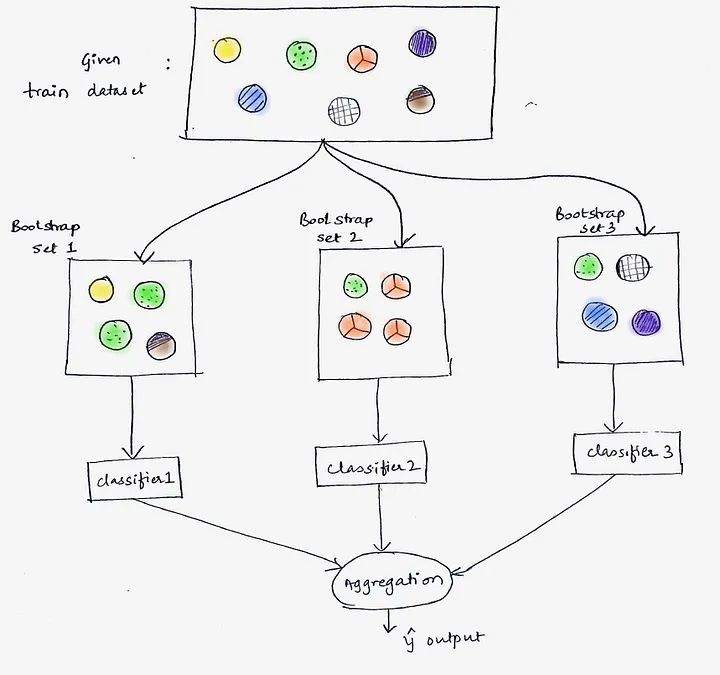
\includegraphics[keepaspectratio]{images/bagging-visualization.png}}
\caption{Bagging Visualization}
\end{figure}

\begin{center}\rule{0.5\linewidth}{0.5pt}\end{center}

\subsection{\texorpdfstring{\textbf{2.
Boosting}}{2. Boosting}}\label{boosting}

\subsubsection{\texorpdfstring{\textbf{Concept:}}{Concept:}}\label{concept-1}

\begin{itemize}
\tightlist
\item
  \textbf{Boosting} focuses on \textbf{reducing bias} by training models
  sequentially, with each model attempting to correct the errors made by
  the previous ones.
\item
  Each subsequent model focuses on the \textbf{misclassified examples}
  from the previous model, making boosting a more \textbf{adaptive}
  method than bagging.
\end{itemize}

\subsubsection{\texorpdfstring{\textbf{How It
Works:}}{How It Works:}}\label{how-it-works-1}

\begin{enumerate}
\def\labelenumi{\arabic{enumi}.}
\tightlist
\item
  \textbf{Sequential Learning:} Models are trained one after the other,
  and each model attempts to fix the mistakes made by the previous
  model.
\item
  \textbf{Weight Assignment:} In boosting, each data point is given a
  weight. Initially, all points have equal weight, but after each round,
  \textbf{misclassified} points are given \textbf{higher weight} so the
  next model focuses more on those errors.
\item
  \textbf{Combining Predictions:} The predictions of all the models are
  combined using a \textbf{weighted sum}. Models that perform well are
  given higher weight in the final prediction.
\end{enumerate}

\subsubsection{\texorpdfstring{\textbf{Key Point:} Models are trained
\textbf{sequentially}, and each model is given \textbf{different
importance} in the final prediction based on its
performance.}{Key Point: Models are trained sequentially, and each model is given different importance in the final prediction based on its performance.}}\label{key-point-models-are-trained-sequentially-and-each-model-is-given-different-importance-in-the-final-prediction-based-on-its-performance.}

\subsubsection{\texorpdfstring{\textbf{Example:}}{Example:}}\label{example-1}

Suppose you are predicting customer churn (whether a customer will leave
a service or not): - Start by training a decision tree on the entire
dataset. If some data points are misclassified, increase their
importance (weight) for the next model. - Train the next model, focusing
more on the data points that were misclassified by the first model. -
Continue this process sequentially and combine the predictions from all
models.

\subsubsection{\texorpdfstring{\textbf{Advantages of
Boosting:}}{Advantages of Boosting:}}\label{advantages-of-boosting}

\begin{itemize}
\tightlist
\item
  \textbf{Reduces bias:} By focusing on the errors of previous models,
  boosting can achieve a high level of accuracy.
\item
  \textbf{Good for complex models:} Boosting works well even with simple
  models like decision stumps (trees with one level) because it builds
  on their weaknesses.
\end{itemize}

\subsubsection{\texorpdfstring{\textbf{Real-world Example: AdaBoost and
Gradient
Boosting}}{Real-world Example: AdaBoost and Gradient Boosting}}\label{real-world-example-adaboost-and-gradient-boosting}

\begin{itemize}
\tightlist
\item
  \textbf{AdaBoost (Adaptive Boosting):} Adjusts the weights of
  misclassified instances and assigns higher importance to models that
  perform well.
\item
  \textbf{Gradient Boosting:} Focuses on reducing the errors in a
  gradient descent fashion by minimizing a loss function iteratively.
\end{itemize}

\subsubsection{\texorpdfstring{\textbf{Visualization:}}{Visualization:}}\label{visualization-1}

\begin{figure}
\centering
\pandocbounded{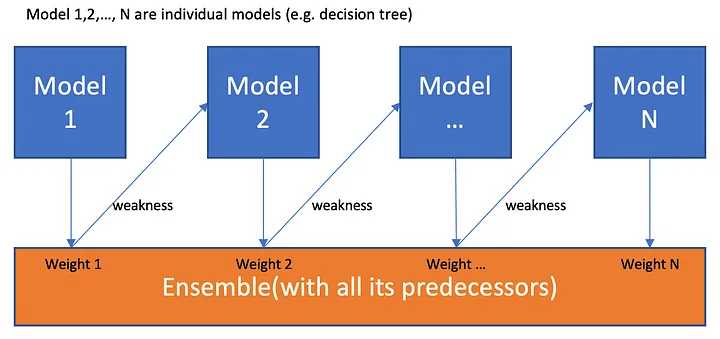
\includegraphics[keepaspectratio]{images/boosting-visualization.png}}
\caption{Boosting Visualization}
\end{figure}

\begin{center}\rule{0.5\linewidth}{0.5pt}\end{center}

\subsection{\texorpdfstring{\textbf{Key Differences Between Bagging and
Boosting}}{Key Differences Between Bagging and Boosting}}\label{key-differences-between-bagging-and-boosting}

\begin{longtable}[]{@{}
  >{\raggedright\arraybackslash}p{(\linewidth - 4\tabcolsep) * \real{0.3333}}
  >{\raggedright\arraybackslash}p{(\linewidth - 4\tabcolsep) * \real{0.3333}}
  >{\raggedright\arraybackslash}p{(\linewidth - 4\tabcolsep) * \real{0.3333}}@{}}
\toprule\noalign{}
\begin{minipage}[b]{\linewidth}\raggedright
Feature
\end{minipage} & \begin{minipage}[b]{\linewidth}\raggedright
\textbf{Bagging}
\end{minipage} & \begin{minipage}[b]{\linewidth}\raggedright
\textbf{Boosting}
\end{minipage} \\
\midrule\noalign{}
\endhead
\bottomrule\noalign{}
\endlastfoot
\textbf{Objective} & Reduce \textbf{variance} by combining multiple
models & Reduce \textbf{bias} by focusing on misclassified instances \\
\textbf{Model Training} & Models are trained \textbf{independently} and
in \textbf{parallel} & Models are trained \textbf{sequentially}, each
learning from the mistakes of the previous one \\
\textbf{Importance of Models} & All models have \textbf{equal weight} in
final prediction & Models have \textbf{different weights} based on
performance \\
\textbf{Data Subsampling} & Each model is trained on a different
\textbf{bootstrapped subset} of the data & Each model is trained on the
\textbf{same dataset}, but misclassified examples get more weight \\
\textbf{Examples of Algorithms} & Random Forest & AdaBoost, Gradient
Boosting, XGBoost \\
\textbf{Best Suited For} & High-variance models like decision trees &
High-bias models like decision stumps \\
\end{longtable}

\begin{center}\rule{0.5\linewidth}{0.5pt}\end{center}

\subsubsection{\texorpdfstring{\textbf{Detailed
Examples}}{Detailed Examples}}\label{detailed-examples}

\subsubsection{\texorpdfstring{\textbf{1. Bagging Example (Random Forest
for
Classification)}}{1. Bagging Example (Random Forest for Classification)}}\label{bagging-example-random-forest-for-classification}

Imagine you are classifying emails as ``spam'' or ``not spam.'' Using
\textbf{Random Forest} (a bagging method): - You create multiple
bootstrapped samples of your email dataset. - Train separate decision
trees on each subset. - Each decision tree classifies the email as
``spam'' or ``not spam.'' - The final decision is based on the
\textbf{majority vote} from all the trees.

Here, each tree operates independently and has equal influence in the
final decision.

\subsubsection{\texorpdfstring{\textbf{2. Boosting Example (AdaBoost for
Classification)}}{2. Boosting Example (AdaBoost for Classification)}}\label{boosting-example-adaboost-for-classification}

Now, consider using \textbf{AdaBoost} for the same email classification
task: - Train a first simple decision tree (called a \textbf{decision
stump}) on the entire dataset. It misclassifies some emails. - Increase
the weights of the misclassified emails so that the next decision stump
pays more attention to them. - Train another decision stump on the
re-weighted data. This stump focuses on correcting the previous stump's
errors. - Repeat this process several times. - Combine the results of
all stumps, but give more weight to the better-performing ones.

Here, the later models learn from the mistakes of the earlier models,
and each model has a different influence on the final output.

\begin{center}\rule{0.5\linewidth}{0.5pt}\end{center}

\subsubsection{\texorpdfstring{\textbf{Conclusion:}}{Conclusion:}}\label{conclusion}

\begin{itemize}
\tightlist
\item
  \textbf{Bagging} is a technique for reducing \textbf{variance} and
  preventing overfitting by training models independently on different
  subsets of data.
\item
  \textbf{Boosting} is a method for reducing \textbf{bias} by training
  models sequentially, where each model focuses on the errors of the
  previous ones.
\end{itemize}

Both methods improve model accuracy, but they are applied in different
scenarios based on whether you're trying to reduce \textbf{variance}
(Bagging) or \textbf{bias} (Boosting).

\begin{longtable}[]{@{}l@{}}
\toprule\noalign{}
\endhead
\bottomrule\noalign{}
\endlastfoot
Boosting \\
\end{longtable}

Boosting is an ensemble machine learning technique that combines the
predictions of multiple weak learners (typically decision trees) to
create a stronger, more accurate model. The key idea behind boosting is
to improve model accuracy by focusing on the errors of previous models
and correcting them iteratively.

Here's a breakdown to help you understand and explain boosting in an
interview:

\subsubsection{\texorpdfstring{1. \textbf{Weak
Learners}}{1. Weak Learners}}\label{weak-learners}

In boosting, each model (or ``learner'') is typically a weak learner,
meaning it performs only slightly better than random guessing. Decision
stumps (trees with just one split) are commonly used as weak learners.
The power of boosting comes from combining many of these weak learners
to form a strong learner.

\subsubsection{\texorpdfstring{2. \textbf{Sequential
Training}}{2. Sequential Training}}\label{sequential-training}

Boosting builds the model sequentially, with each new learner focusing
on the mistakes (errors) made by the previous learners. The key is that
later models in the sequence are trained to pay more attention to data
points that the earlier models misclassified.

\subsubsection{\texorpdfstring{3.
\textbf{Weighting}}{3. Weighting}}\label{weighting}

At each step, boosting adjusts the weights of the training data points.
The data points that were misclassified in previous models are given
higher weights, meaning the next model in the sequence will focus more
on those hard-to-classify points. This process continues iteratively,
with each model improving upon the errors of the last.

\subsubsection{\texorpdfstring{4. \textbf{Final
Prediction}}{4. Final Prediction}}\label{final-prediction}

In the final model, the predictions from all the learners are combined.
The combination can be a weighted sum (for regression) or a majority
vote (for classification). Because each learner focuses on different
aspects of the data, their combined predictions are more accurate than
any individual learner.

\subsubsection{\texorpdfstring{5. \textbf{Key Boosting
Algorithms}}{5. Key Boosting Algorithms}}\label{key-boosting-algorithms}

\begin{itemize}
\tightlist
\item
  \textbf{AdaBoost (Adaptive Boosting)}: One of the earliest and
  simplest boosting algorithms. It adjusts the weights of misclassified
  points and combines models based on their accuracy.
\item
  \textbf{Gradient Boosting}: This method builds models in a way that
  minimizes the residual errors (the difference between actual and
  predicted values). It uses gradient descent to optimize the loss
  function.
\item
  \textbf{XGBoost and LightGBM}: These are advanced versions of Gradient
  Boosting that improve efficiency and scalability, commonly used in
  practice.
\end{itemize}

\subsubsection{Example for Explaining in an
Interview:}\label{example-for-explaining-in-an-interview}

\begin{itemize}
\tightlist
\item
  Think of boosting like a group project. Each team member (weak
  learner) contributes their part, and if one member makes a mistake,
  the next one steps in to correct it. Over time, the group produces a
  much better result than any individual could have on their own.
\end{itemize}

\subsubsection{Key Benefits of
Boosting:}\label{key-benefits-of-boosting}

\begin{itemize}
\tightlist
\item
  \textbf{Accuracy}: It often yields state-of-the-art performance,
  especially in structured/tabular data.
\item
  \textbf{Flexibility}: Can handle both classification and regression
  tasks.
\item
  \textbf{Focus on Errors}: By emphasizing the hardest-to-classify
  examples, boosting can achieve a high level of precision.
\end{itemize}

\subsubsection{Limitations:}\label{limitations}

\begin{itemize}
\tightlist
\item
  \textbf{Overfitting}: Boosting can overfit if not properly
  regularized, especially with noisy data.
\item
  \textbf{Computationally Intensive}: Sequential training can be slow
  for large datasets or complex models.
\end{itemize}

If you can explain it this way, focusing on its sequential correction
mechanism and its effectiveness at creating strong models from weak
learners, you'll give a solid and clear explanation in your interview.

\begin{longtable}[]{@{}l@{}}
\toprule\noalign{}
\endhead
\bottomrule\noalign{}
\endlastfoot
Ada Boosting \\
\end{longtable}

\subsubsection{AdaBoost Algorithm - Explained
Mathematically}\label{adaboost-algorithm---explained-mathematically}

AdaBoost (short for \textbf{Adaptive Boosting}) is a popular boosting
algorithm designed to combine multiple weak classifiers into a single
strong classifier. Its main idea is to iteratively adjust the weights of
misclassified points, focusing on the harder-to-classify instances in
each round. Here's a deep yet simple explanation, starting from the math
behind it.

\paragraph{Step-by-Step Breakdown}\label{step-by-step-breakdown}

\begin{enumerate}
\def\labelenumi{\arabic{enumi}.}
\item
  \textbf{Initialize Weights}\\
  We start by giving each training example an equal weight. If we have
  \texttt{n} training samples, then each sample gets an initial weight:

  \[
  w_1(i) = \frac{1}{n}
  \] where \(( w_1(i) )\) is the weight of the \((i)\)-th example at the
  first iteration.
\item
  \textbf{Train the First Weak Classifier}\\
  At each iteration, train a weak classifier \((h_t(x))\) (usually a
  decision stump) on the dataset, with weighted data points. The weak
  classifier's goal is to minimize the weighted classification error.
  The weighted error of the weak classifier \((h_t(x))\) is calculated
  as:

  \[
  \epsilon_t = \frac{\sum_{i=1}^{n} {w_t(i) \cdot {1}(h_t(x_i) \neq y_i)}}{\sum_{i=1}^{n} w_t(i)}
  \] where:

  \begin{itemize}
  \tightlist
  \item
    \(( w_t(i) )\) is the weight of the \((i)\)-th sample at iteration
    \((t)\),
  \item
    \(( h_t(x_i) )\) is the prediction of the weak classifier for the
    \((i)\)-th sample,
  \item
    \(( y_i )\) is the true label of the \((i)\)-th sample,
  \item
    \( {1}(h_t(x_i) \neq y_i) \) is an indicator function (1 if
    the classifier was wrong, 0 if correct).
  \end{itemize}
\item
  \textbf{Compute Classifier Weight (Alpha)}\\
  The algorithm assigns a weight \(( \alpha_t )\) to the weak classifier
  based on its performance. A classifier that performs well (low error
  rate) gets a higher weight, and a classifier that performs poorly gets
  a lower weight. The weight is calculated as:

  \[
  \alpha_t = \frac{1}{2} \ln\left(\frac{1 - \epsilon_t}{\epsilon_t}\right)
  \]

  \begin{itemize}
  \tightlist
  \item
    If the classifier is perfect, \(( \epsilon_t = 0 )\), then
    \(( \alpha_t )\) becomes large, emphasizing that classifier.
  \item
    If \(( \epsilon_t = 0.5 )\) (random guessing), \(( \alpha_t = 0 )\),
    meaning that classifier contributes nothing.
  \end{itemize}
\item
  \textbf{Update Weights}\\
  After each weak classifier, the weights of the misclassified samples
  are increased so that the next classifier focuses more on the
  hard-to-classify points. The updated weight for the next iteration is:

  \[
  w_{t+1}(i) = w_t(i) \cdot \exp(\alpha_t \cdot {1}(h_t(x_i) \neq y_i))
  \]

  This means:

  \begin{itemize}
  \tightlist
  \item
    If the classifier predicts correctly, the weight of that sample
    decreases.
  \item
    If it predicts incorrectly, the weight of that sample increases,
    forcing the next classifier to focus more on that misclassified
    point.
  \end{itemize}

  Finally, we normalize the weights so that they sum up to 1:

  \[
  w_{t+1}(i) = \frac{w_{t+1}(i)}{\sum_{i=1}^{n} w_{t+1}(i)}
  \]
\item
  \textbf{Final Prediction}\\
  After multiple iterations, AdaBoost combines the weak classifiers into
  a strong classifier. The final prediction is a weighted vote of all
  the weak classifiers, where each classifier's vote is weighted by its
  corresponding \(( \alpha_t )\):

  \[
  H(x) = \text{sign}\left(\sum_{t=1}^{T} \alpha_t h_t(x)\right)
  \]

  \begin{itemize}
  \tightlist
  \item
    If the sum of weighted predictions is positive, \((H(x) = 1)\),
    otherwise \((H(x) = -1)\) (for binary classification).
  \end{itemize}
\end{enumerate}

\begin{center}\rule{0.5\linewidth}{0.5pt}\end{center}

\subsubsection{Simplified Explanation (For
Interviews)}\label{simplified-explanation-for-interviews}

Here's how you can explain AdaBoost in an interview in a simple and
intuitive way:

\begin{enumerate}
\def\labelenumi{\arabic{enumi}.}
\item
  \textbf{Boosting Concept}\\
  Imagine you're assembling a team of students to solve a complex math
  problem. Each student is good at solving certain types of questions
  but struggles with others. After each round, you notice which student
  made mistakes and ask the next student to focus more on those problem
  areas. Over time, their combined effort leads to a much better
  solution than any one student could achieve alone.
\item
  \textbf{AdaBoost's Step-by-Step Approach}

  \begin{itemize}
  \tightlist
  \item
    \textbf{Start with Equal Importance}: In the beginning, all your
    training data points are treated equally.
  \item
    \textbf{Focus on Mistakes}: After training a simple model, you look
    at where it went wrong. In the next round, you focus more on those
    harder cases.
  \item
    \textbf{Combine Weak Models}: You repeat this process multiple
    times, and at the end, you combine the results from all models to
    make a strong final prediction.
  \end{itemize}
\item
  \textbf{How It Works}\\
  AdaBoost works by adjusting the importance (weight) of each data
  point. It assigns higher importance to data points that are
  misclassified and gives more weight to models that perform well. The
  algorithm improves iteratively, focusing more and more on the
  difficult examples.
\item
  \textbf{Final Decision}\\
  The final model is a combination of all the weak models. It makes
  decisions based on a weighted vote, where models that performed better
  have more influence on the final outcome.
\end{enumerate}

\begin{center}\rule{0.5\linewidth}{0.5pt}\end{center}

\subsubsection{Key Points to Remember for the
Interview}\label{key-points-to-remember-for-the-interview}

\begin{itemize}
\tightlist
\item
  \textbf{AdaBoost builds a model sequentially}, with each new model
  improving the errors made by the previous ones.
\item
  \textbf{Weights are updated} to focus on misclassified points, so the
  algorithm adapts and becomes more accurate with each iteration.
\item
  \textbf{The final model is a weighted sum of weak models}, making
  AdaBoost powerful despite using weak learners like decision stumps.
\end{itemize}

This mathematical explanation and simplified approach should give you a
solid foundation to both understand and explain AdaBoost clearly and
effectively!

\begin{longtable}[]{@{}l@{}}
\toprule\noalign{}
\endhead
\bottomrule\noalign{}
\endlastfoot
Gradient Boosting \\
\end{longtable}

\subsubsection{Gradient Boosting Algorithm: Mathematical
Explanation}\label{gradient-boosting-algorithm-mathematical-explanation}

\textbf{Gradient Boosting} is an ensemble machine learning technique
that builds a strong predictive model by combining the outputs of
multiple weak learners (typically decision trees). The key difference
from AdaBoost is that \textbf{Gradient Boosting} uses a gradient descent
approach to minimize the error or loss function. It builds models
sequentially, where each new model tries to correct the errors
(residuals) made by the previous models.

Let's break down Gradient Boosting mathematically so you can develop a
deep understanding and explain it in an easy way.

\begin{center}\rule{0.5\linewidth}{0.5pt}\end{center}

\subsubsection{\texorpdfstring{1. \textbf{Key
Concept}:}{1. Key Concept:}}\label{key-concept}

Gradient Boosting focuses on optimizing a loss function by iteratively
adding models that correct the previous models' errors.

Mathematically, it aims to minimize a loss function
\(( L(y, \hat{y}) )\), where: - \(( y )\) is the true target value, -
\(( \hat{y} )\) is the predicted value.

\begin{center}\rule{0.5\linewidth}{0.5pt}\end{center}

\subsubsection{Step-by-Step Explanation of Gradient
Boosting:}\label{step-by-step-explanation-of-gradient-boosting}

\begin{enumerate}
\def\labelenumi{\arabic{enumi}.}
\item
  \textbf{Initialization}:\\
  The algorithm starts with a constant model that minimizes the loss
  function. For regression, this is often the mean value of the target
  variable \(( y )\).

  \[
  F_0(x) = \arg \min_{\gamma} \sum_{i=1}^{n} L(y_i, \gamma)
  \]

  \begin{itemize}
  \tightlist
  \item
    \(( F_0(x) )\) is the initial prediction (like a baseline model),
  \item
    \(( L(y_i, \gamma) )\) is the loss function (e.g., squared error,
    absolute error).
  \end{itemize}

  For example, in regression with squared error loss, the best constant
  prediction is the mean of the target variable \(( y )\).
\end{enumerate}

\begin{center}\rule{0.5\linewidth}{0.5pt}\end{center}

\begin{enumerate}
\def\labelenumi{\arabic{enumi}.}
\setcounter{enumi}{1}
\item
  \textbf{Training Multiple Trees Iteratively}:\\
  At each iteration \(( t )\), the goal is to add a new weak learner
  \(( h_t(x) )\) that helps reduce the residual errors of the current
  model \(( F_t(x) )\). The current model at iteration \(( t )\) is:

  \[
  F_t(x) = F_{t-1}(x) + \nu \cdot h_t(x)
  \]

  Here:

  \begin{itemize}
  \tightlist
  \item
    \(( F_t(x) )\) is the model after iteration \(( t )\),
  \item
    \(( F_{t-1}(x) )\) is the previous model,
  \item
    \(( h_t(x) )\) is the weak learner (decision tree) added in the
    \(( t )\)-th iteration,
  \item
    \(( \nu )\) is the learning rate, a parameter that controls how much
    we adjust the previous model.
  \end{itemize}
\end{enumerate}

\begin{center}\rule{0.5\linewidth}{0.5pt}\end{center}

\begin{enumerate}
\def\labelenumi{\arabic{enumi}.}
\setcounter{enumi}{2}
\item
  \textbf{Residuals}:\\
  Each weak learner \(( h_t(x) )\) is trained to fit the
  \textbf{residuals} (the difference between the actual values \(( y )\)
  and the current prediction \(( F_{t-1}(x) )\)) from the previous
  model:

  \[
  r_{ti} = - \frac{\partial L(y_i, F_{t-1}(x_i))}{\partial F_{t-1}(x_i)}
  \]

  \begin{itemize}
  \tightlist
  \item
    \(( r_{ti} )\) represents the residuals for the \(( i )\)-th data
    point at iteration \(( t )\),
  \item
    The residuals are the \textbf{negative gradient} of the loss
    function with respect to the current model's predictions.
  \end{itemize}

  In simple terms, at each step, Gradient Boosting tries to minimize how
  wrong the current model is by learning a new model that predicts the
  residuals.
\end{enumerate}

\begin{center}\rule{0.5\linewidth}{0.5pt}\end{center}

\begin{enumerate}
\def\labelenumi{\arabic{enumi}.}
\setcounter{enumi}{3}
\tightlist
\item
  \textbf{Fitting the Weak Learner}:\\
  Once the residuals are computed, the next step is to fit a new weak
  learner \(( h_t(x) )\) (usually a decision tree) to these residuals.
  This learner predicts how to adjust the current model to reduce the
  residuals (errors).
\end{enumerate}

\begin{center}\rule{0.5\linewidth}{0.5pt}\end{center}

\begin{enumerate}
\def\labelenumi{\arabic{enumi}.}
\setcounter{enumi}{4}
\item
  \textbf{Updating the Model}:\\
  After the weak learner \(( h_t(x) )\) is trained, the model is updated
  as:

  \[
  F_t(x) = F_{t-1}(x) + \nu \cdot h_t(x)
  \]

  \begin{itemize}
  \tightlist
  \item
    \(( \nu )\) (the learning rate) controls the contribution of the
    weak learner \(( h_t(x) )\) to the final model. Smaller values of
    \(( \nu )\) make the learning process slower but often lead to
    better generalization.
  \end{itemize}
\end{enumerate}

\begin{center}\rule{0.5\linewidth}{0.5pt}\end{center}

\begin{enumerate}
\def\labelenumi{\arabic{enumi}.}
\setcounter{enumi}{5}
\item
  \textbf{Final Model}:\\
  After \(( T )\) iterations, the final prediction is a sum of the
  initial prediction \(( F_0(x) )\) and all the weak learners
  \(( h_t(x) )\):

  \[
  F_T(x) = F_0(x) + \sum_{t=1}^{T} \nu \cdot h_t(x)
  \]

  \begin{itemize}
  \tightlist
  \item
    \(( F_T(x) )\) is the final model after \(( T )\) iterations.
  \end{itemize}
\end{enumerate}

\begin{center}\rule{0.5\linewidth}{0.5pt}\end{center}

\subsubsection{Mathematical Example for
Regression:}\label{mathematical-example-for-regression}

Let's assume we are doing \textbf{regression} and our loss function is
\textbf{mean squared error}
\(( L(y, F(x)) = \frac{1}{2}(y - F(x))^2 )\). Here's how Gradient
Boosting works step by step in this case:

\begin{enumerate}
\def\labelenumi{\arabic{enumi}.}
\item
  \textbf{Initialize}:\\
  Start with an initial guess (e.g., the mean of the target variable
  \(( y )\)):

  \[
  F_0(x) = \frac{1}{n} \sum_{i=1}^{n} y_i
  \]
\item
  \textbf{Compute Residuals}:\\
  At iteration \(( t )\), compute the residuals:

  \[
  r_{ti} = y_i - F_{t-1}(x_i)
  \]
\item
  \textbf{Fit Weak Learner}:\\
  Fit a weak learner \(( h_t(x) )\) to the residuals:

  \[
  h_t(x) \approx r_{ti}
  \]
\item
  \textbf{Update the Model}:\\
  Update the model with the weak learner's prediction:

  \[
  F_t(x) = F_{t-1}(x) + \nu \cdot h_t(x)
  \]
\end{enumerate}

Repeat the steps for multiple iterations until the model converges or
reaches a predetermined number of iterations.

\begin{center}\rule{0.5\linewidth}{0.5pt}\end{center}

\subsubsection{Simplified Explanation for
Interviews:}\label{simplified-explanation-for-interviews-1}

If you're explaining this in an interview, here's a simplified version:

\begin{enumerate}
\def\labelenumi{\arabic{enumi}.}
\tightlist
\item
  \textbf{Concept}:

  \begin{itemize}
  \tightlist
  \item
    Gradient Boosting works by sequentially adding models that correct
    the errors of previous models.
  \item
    At each step, it trains a weak model (like a small decision tree) to
    predict the errors (or residuals) made by the current model.
  \end{itemize}
\item
  \textbf{Optimization via Gradients}:

  \begin{itemize}
  \tightlist
  \item
    The algorithm uses the concept of \textbf{gradient descent}: it
    optimizes the model by minimizing the loss function.
  \item
    Instead of fitting the target variable directly, Gradient Boosting
    fits the negative gradient of the loss (which is the direction in
    which the model needs to improve).
  \end{itemize}
\item
  \textbf{Learning Rate}:

  \begin{itemize}
  \tightlist
  \item
    The learning rate controls how big of a step we take in each
    iteration. A smaller learning rate usually leads to better results
    but requires more iterations.
  \end{itemize}
\item
  \textbf{Final Model}:

  \begin{itemize}
  \tightlist
  \item
    The final model is just the sum of all these weak models, each one
    slightly improving the accuracy.
  \end{itemize}
\end{enumerate}

\begin{center}\rule{0.5\linewidth}{0.5pt}\end{center}

\subsubsection{Key Differences from
AdaBoost:}\label{key-differences-from-adaboost}

\begin{itemize}
\tightlist
\item
  \textbf{Gradient Boosting} minimizes a loss function (like squared
  error or log loss) using \textbf{gradient descent}, focusing on
  reducing residuals.
\item
  \textbf{AdaBoost} adjusts the weights of data points based on
  classification errors, focusing more on misclassified points.
\end{itemize}

\begin{center}\rule{0.5\linewidth}{0.5pt}\end{center}

\subsubsection{Key Takeaways:}\label{key-takeaways}

\begin{itemize}
\tightlist
\item
  \textbf{Gradient Boosting} is a powerful, flexible method that works
  well in practice, especially with structured/tabular data.
\item
  \textbf{Weak learners} (usually decision trees) are added
  sequentially, each one focusing on correcting the mistakes of the
  previous ones.
\item
  \textbf{Learning rate} and \textbf{number of iterations} are crucial
  parameters. A smaller learning rate typically requires more iterations
  but results in better generalization.
\end{itemize}

If you explain it this way in an interview, you'll convey both the
intuition and the mathematical foundation of the Gradient Boosting
algorithm effectively!

\begin{longtable}[]{@{}l@{}}
\toprule\noalign{}
\endhead
\bottomrule\noalign{}
\endlastfoot
XGBoost \\
\end{longtable}

\subsubsection{XGBoost (Extreme Gradient Boosting): Explanation with
Equations and
Formulas}\label{xgboost-extreme-gradient-boosting-explanation-with-equations-and-formulas}

\textbf{XGBoost} (e\textbf{X}treme \textbf{G}radient \textbf{Boost}ing)
is an advanced implementation of the Gradient Boosting algorithm. It is
widely used due to its performance, efficiency, and scalability,
especially for structured/tabular data. XGBoost is known for
regularization, handling missing values, and parallelization, which
makes it faster and more accurate than traditional Gradient Boosting
methods.

Let's break down XGBoost both mathematically and conceptually so you can
understand and explain it easily.

\begin{center}\rule{0.5\linewidth}{0.5pt}\end{center}

\subsubsection{\texorpdfstring{1. \textbf{Key Concept of
XGBoost:}}{1. Key Concept of XGBoost:}}\label{key-concept-of-xgboost}

XGBoost builds a model \textbf{sequentially} by adding \textbf{weak
learners} (typically decision trees) to minimize a given \textbf{loss
function}. It focuses on \textbf{residuals} (errors) at each stage and
uses a second-order Taylor expansion to optimize the loss, which
differentiates it from traditional Gradient Boosting.

XGBoost can handle regression, binary, and multi-class classification
problems by using different loss functions (e.g., squared error for
regression, log loss for classification).

\begin{center}\rule{0.5\linewidth}{0.5pt}\end{center}

\subsubsection{\texorpdfstring{2. \textbf{Mathematical Framework of
XGBoost:}}{2. Mathematical Framework of XGBoost:}}\label{mathematical-framework-of-xgboost}

\paragraph{Objective Function}\label{objective-function}

The objective function in XGBoost consists of two parts: 1. \textbf{Loss
Function} \(( L(\theta) )\): Measures how well the model fits the
training data. 2. \textbf{Regularization Term} \(( \Omega(f) )\):
Controls the complexity of the model to prevent overfitting.

The goal is to minimize the objective function \(( Obj(\theta) )\):

\[
Obj(\theta) = \sum_{i=1}^{n} L(y_i, \hat{y}_i) + \sum_{k=1}^{K} \Omega(f_k)
\]

Where: - \(( n )\) is the number of training examples, - \(( y_i )\) is
the true label, - \(( \hat{y}_i )\) is the predicted value from the
model, - \(( K )\) is the number of weak learners (trees), -
\(( L(y_i, \hat{y}_i) )\) is the loss function (e.g., squared error or
log loss), - \(( \Omega(f_k) )\) is the regularization term that
penalizes the complexity of the \(( k )\)-th weak learner.

For decision trees, the regularization term \(( \Omega(f_k) )\) is
defined as:

\[
\Omega(f) = \gamma T + \frac{1}{2} \lambda \sum_{j=1}^{T} w_j^2
\]

Where: - \(( T )\) is the number of leaves in the tree, - \(( w_j )\) is
the weight assigned to the \(( j )\)-th leaf, - \(( \gamma )\) is a
regularization parameter that penalizes the number of leaves (controls
the tree size), - \(( \lambda )\) is a regularization parameter that
penalizes large weights (controls overfitting).

\begin{center}\rule{0.5\linewidth}{0.5pt}\end{center}

\subsubsection{\texorpdfstring{3. \textbf{Additive
Model:}}{3. Additive Model:}}\label{additive-model}

In XGBoost, we add one weak learner (tree) at each iteration to improve
the model. The predicted value after \(( t )\) trees is:

\[
\hat{y}_i^{(t)} = \hat{y}_i^{(t-1)} + f_t(x_i)
\]

Where: - \(( \hat{y}_i^{(t)} )\) is the prediction for the \(( i )\)-th
instance after \(( t )\) iterations, - \(( \hat{y}_i^{(t-1)} )\) is the
prediction after \(( t-1 )\) iterations, - \(( f_t(x_i) )\) is the
prediction from the \(( t )\)-th tree.

The goal is to find the function \(( f_t(x_i) )\) (the next tree) that
minimizes the overall loss.

\begin{center}\rule{0.5\linewidth}{0.5pt}\end{center}

\subsubsection{\texorpdfstring{4. \textbf{Taylor Expansion for
Approximation:}}{4. Taylor Expansion for Approximation:}}\label{taylor-expansion-for-approximation}

XGBoost uses \textbf{second-order Taylor expansion} to approximate the
objective function, making the optimization more efficient. The loss
function \(( L(y_i, \hat{y}_i) )\) is expanded as:

\[
L(y_i, \hat{y}_i + f_t(x_i)) \approx L(y_i, \hat{y}_i) + g_i f_t(x_i) + \frac{1}{2} h_i f_t(x_i)^2
\]

Where: -
\(( g_i = \frac{\partial L(y_i, \hat{y}_i)}{\partial \hat{y}_i} )\) (the
first derivative, or \textbf{gradient}), -
\(( h_i = \frac{\partial^2 L(y_i, \hat{y}_i)}{\partial \hat{y}_i^2} )\)
(the second derivative, or \textbf{Hessian}).

This second-order approximation allows the algorithm to update the model
more accurately at each iteration, using both the gradient (first
derivative) and curvature (second derivative) information.

\begin{center}\rule{0.5\linewidth}{0.5pt}\end{center}

\subsubsection{\texorpdfstring{5. \textbf{Tree
Building:}}{5. Tree Building:}}\label{tree-building}

At each iteration, XGBoost builds a new decision tree by minimizing the
following \textbf{objective function}:

\[
Obj = \sum_{i=1}^{n} \left( g_i f_t(x_i) + \frac{1}{2} h_i f_t(x_i)^2 \right) + \Omega(f_t)
\]

The model chooses the best split for the tree by optimizing this
objective function. Specifically, the \textbf{Gain} from a split is
computed as:

\[
Gain = \frac{1}{2} \left( \frac{G_L^2}{H_L + \lambda} + \frac{G_R^2}{H_R + \lambda} - \frac{(G_L + G_R)^2}{H_L + H_R + \lambda} \right) - \gamma
\]

Where: - \(( G_L )\) and \(( G_R )\) are the sums of gradients for the
left and right nodes, respectively, - \(( H_L )\) and \(( H_R )\) are
the sums of Hessians for the left and right nodes, respectively, -
\(( \lambda )\) and \(( \gamma )\) are regularization parameters.

This \textbf{Gain} measures how much a split improves the model by
separating the data into more homogeneous groups (with similar target
values).

The tree is built recursively by maximizing the Gain at each step, and
the process stops when the Gain becomes smaller than a predefined
threshold.

\begin{center}\rule{0.5\linewidth}{0.5pt}\end{center}

\subsubsection{\texorpdfstring{6. \textbf{Regularization in
XGBoost:}}{6. Regularization in XGBoost:}}\label{regularization-in-xgboost}

XGBoost introduces \textbf{regularization} to control the complexity of
the trees and prevent overfitting. This includes:

\begin{itemize}
\tightlist
\item
  \textbf{\(( \lambda )\)}: L2 regularization term on leaf weights to
  reduce the influence of high weights.
\item
  \textbf{\(( \gamma )\)}: Penalty for the number of leaves in the tree
  to prevent overly complex trees.
\end{itemize}

These regularization terms help improve the generalization of the model
by penalizing trees that are too complex.

\begin{center}\rule{0.5\linewidth}{0.5pt}\end{center}

\subsubsection{\texorpdfstring{7. \textbf{Shrinkage (Learning
Rate):}}{7. Shrinkage (Learning Rate):}}\label{shrinkage-learning-rate}

In XGBoost, the \textbf{learning rate} \(( \eta )\) (also called
\textbf{shrinkage}) controls how much each tree contributes to the final
prediction:

\[
\hat{y}_i^{(t)} = \hat{y}_i^{(t-1)} + \eta f_t(x_i)
\]

Where: - \(( \eta \in (0, 1] )\) is the learning rate.

A smaller learning rate means that each tree has less impact, but the
model generally requires more trees to converge.

\begin{center}\rule{0.5\linewidth}{0.5pt}\end{center}

\subsubsection{\texorpdfstring{8. \textbf{Handling Missing
Values:}}{8. Handling Missing Values:}}\label{handling-missing-values}

XGBoost can handle missing values by learning the optimal direction
(left or right) for missing data in each split. When a feature value is
missing for a data point, XGBoost assigns it to a default direction
based on Gain.

\begin{center}\rule{0.5\linewidth}{0.5pt}\end{center}

\subsubsection{\texorpdfstring{9. \textbf{Parallelization and
Efficiency:}}{9. Parallelization and Efficiency:}}\label{parallelization-and-efficiency}

XGBoost is highly efficient because it: - \textbf{Parallelizes tree
construction} by splitting data across different threads, - Uses
\textbf{column block compression} to optimize memory usage and speed up
computation.

\begin{center}\rule{0.5\linewidth}{0.5pt}\end{center}

\subsubsection{Simplified Explanation for
Interviews:}\label{simplified-explanation-for-interviews-2}

If you're explaining XGBoost in an interview, here's a simpler version:

\begin{enumerate}
\def\labelenumi{\arabic{enumi}.}
\tightlist
\item
  \textbf{Core Idea}:

  \begin{itemize}
  \tightlist
  \item
    XGBoost is an improved version of Gradient Boosting that optimizes
    the loss function using both the first and second derivatives of the
    loss function (Taylor expansion).
  \item
    At each step, it builds a decision tree to correct the errors made
    by the previous trees, aiming to minimize the residual errors.
  \end{itemize}
\item
  \textbf{Efficiency}:

  \begin{itemize}
  \tightlist
  \item
    XGBoost is fast and efficient because it uses advanced techniques
    like second-order optimization (gradient + curvature),
    regularization to prevent overfitting, and parallelization to speed
    up computation.
  \end{itemize}
\item
  \textbf{Regularization}:

  \begin{itemize}
  \tightlist
  \item
    Regularization (L2 and tree pruning) helps prevent overfitting,
    ensuring the model generalizes well to unseen data.
  \end{itemize}
\item
  \textbf{Handling Missing Data}:

  \begin{itemize}
  \tightlist
  \item
    XGBoost handles missing values efficiently by automatically learning
    which direction to send missing data in decision trees.
  \end{itemize}
\item
  \textbf{Learning Rate}:

  \begin{itemize}
  \tightlist
  \item
    The learning rate controls how much each tree contributes to the
    overall model. Smaller learning rates lead to more accurate models
    but require more trees.
  \end{itemize}
\end{enumerate}

\begin{center}\rule{0.5\linewidth}{0.5pt}\end{center}

\subsubsection{Key Takeaways:}\label{key-takeaways-1}

\begin{itemize}
\tightlist
\item
  \textbf{XGBoost} is an advanced form of Gradient Boosting that uses
  second-order Taylor expansion to optimize the loss function.
\item
  It adds decision trees sequentially to correct the residuals (errors)
  from the previous trees.
\item
  \textbf{Regularization}, \textbf{learning rate}, and
  \textbf{parallelization} are key aspects that make XGBoost both
  powerful and efficient.
\item
  XGBoost can handle missing values and large datasets, making it one of
  the best choices for structured/tabular data in many machine learning
\end{itemize}

\begin{longtable}[]{@{}l@{}}
\toprule\noalign{}
\endhead
\bottomrule\noalign{}
\endlastfoot
Loss Function of XGBoost \\
\end{longtable}

The loss function in XGBoost is the mechanism that guides the
optimization process during training by measuring the difference between
predicted and actual values. In XGBoost, the loss function can vary
depending on the type of task (regression, classification, etc.), but it
generally consists of two parts:

\begin{enumerate}
\def\labelenumi{\arabic{enumi}.}
\tightlist
\item
  \textbf{Prediction Loss (Primary Loss Function)}: This represents how
  well the model's predictions match the true labels or target values.
  Common loss functions include:

  \begin{itemize}
  \tightlist
  \item
    \textbf{Regression}:

    \begin{itemize}
    \tightlist
    \item
      \textbf{Mean Squared Error (MSE)}: Used when predicting continuous
      values. \[
      L(y, \hat{y}) = \frac{1}{n} \sum_{i=1}^{n} (y_i - \hat{y}_i)^2
      \]
    \item
      \textbf{Mean Absolute Error (MAE)}: Another option for regression
      tasks.
    \end{itemize}
  \item
    \textbf{Binary Classification}:

    \begin{itemize}
    \tightlist
    \item
      \textbf{Logistic Loss (Log Loss)}: Used in binary classification
      tasks. \[
      L(y, \hat{y}) = -\frac{1}{n} \sum_{i=1}^{n} \left[ y_i \log (\hat{y}_i) + (1 - y_i) \log (1 - \hat{y}_i) \right]
      \]
    \end{itemize}
  \item
    \textbf{Multiclass Classification}:

    \begin{itemize}
    \tightlist
    \item
      \textbf{Softmax Loss}: Extends logistic loss for multiclass
      problems.
    \end{itemize}
  \end{itemize}
\item
  \textbf{Regularization (Penalty)}: XGBoost also includes a
  regularization term to prevent overfitting by penalizing complex
  models. The regularization term consists of:

  \begin{itemize}
  \tightlist
  \item
    \textbf{L1 regularization} (Lasso) on the weights, encouraging
    sparsity (i.e., many weights to be zero).
  \item
    \textbf{L2 regularization} (Ridge) on the weights, which helps
    reduce the magnitude of the weights.
  \end{itemize}
\end{enumerate}

The complete objective function for XGBoost is: \[
\text{Obj} = \sum L(y, \hat{y}) + \text{regularization term}
\] Where: - \((L(y, \hat{y}))\) is the loss function that measures
prediction error. - The regularization term adds constraints to reduce
model complexity.

XGBoost optimizes this objective function using gradient boosting.
During each iteration, it minimizes the loss function by building a new
weak learner (typically a decision tree) that corrects the residuals of
the current model.

\begin{center}\rule{0.5\linewidth}{0.5pt}\end{center}

\subsubsection{Hyperparameters for
XGBoost}\label{hyperparameters-for-xgboost}

XGBoost (Extreme Gradient Boosting) is a powerful implementation of
gradient boosting, offering a range of hyperparameters to fine-tune for
optimal performance. These hyperparameters can be grouped into
categories based on their function: \textbf{general parameters},
\textbf{booster parameters}, \textbf{learning task parameters}, and
\textbf{command-line parameters}. Below is a detailed list:

\begin{center}\rule{0.5\linewidth}{0.5pt}\end{center}

\subsubsection{\texorpdfstring{\textbf{1. General
Parameters}}{1. General Parameters}}\label{general-parameters}

These parameters control the overall behavior of the model.

\begin{itemize}
\item
  \textbf{\texttt{booster}}\strut \\
  Specifies the type of boosting model to use:

  \begin{itemize}
  \tightlist
  \item
    \texttt{"gbtree"} (default): Gradient-boosted trees.
  \item
    \texttt{"gblinear"}: Linear booster (for linear models).
  \item
    \texttt{"dart"}: Dropouts meet Multiple Additive Regression Trees
    (DART).
  \end{itemize}
\item
  \textbf{\texttt{nthread}}\strut \\
  Number of parallel threads to use. Default depends on your system.
\item
  \textbf{\texttt{verbosity}}\strut \\
  Controls the amount of information displayed during training:

  \begin{itemize}
  \tightlist
  \item
    \texttt{0}: Silent.
  \item
    \texttt{1}: Warning (default).
  \item
    \texttt{2}: Info.
  \item
    \texttt{3}: Debug.
  \end{itemize}
\item
  \textbf{\texttt{seed}}\strut \\
  Random seed for reproducibility.
\end{itemize}

\begin{center}\rule{0.5\linewidth}{0.5pt}\end{center}

\subsubsection{\texorpdfstring{\textbf{2. Booster
Parameters}}{2. Booster Parameters}}\label{booster-parameters}

These control the specific behavior of the chosen booster.

\paragraph{\texorpdfstring{\textbf{(a) Tree Booster Parameters
(\texttt{gbtree},
\texttt{dart})}}{(a) Tree Booster Parameters (gbtree, dart)}}\label{a-tree-booster-parameters-gbtree-dart}

\begin{itemize}
\item
  \textbf{\texttt{eta}} (Learning Rate)\\
  Reduces the contribution of each tree. Typical range:
  \texttt{0.01}--\texttt{0.3}.
\item
  \textbf{\texttt{max\_depth}}\strut \\
  Maximum depth of a tree. Higher values lead to more complex models.
  Default: \texttt{6}.
\item
  \textbf{\texttt{min\_child\_weight}}\strut \\
  Minimum sum of instance weights (hessian) needed in a child node.
  Larger values prevent overfitting.
\item
  \textbf{\texttt{gamma}}\strut \\
  Minimum loss reduction required to make a further split. Higher values
  make the algorithm more conservative.
\item
  \textbf{\texttt{subsample}}\strut \\
  Fraction of samples used for training each tree. Range:
  \texttt{(0,\ 1{]}}. Default: \texttt{1.0}.
\item
  \textbf{\texttt{colsample\_bytree}}\strut \\
  Fraction of features used for training each tree. Range:
  \texttt{(0,\ 1{]}}. Default: \texttt{1.0}.
\item
  \textbf{\texttt{colsample\_bylevel}}\strut \\
  Fraction of features used per level of the tree. Default:
  \texttt{1.0}.
\item
  \textbf{\texttt{colsample\_bynode}}\strut \\
  Fraction of features used per split. Default: \texttt{1.0}.
\item
  \textbf{\texttt{lambda}} (L2 Regularization)\\
  Regularization term on leaf weights. Default: \texttt{1}.
\item
  \textbf{\texttt{alpha}} (L1 Regularization)\\
  L1 regularization term on leaf weights. Default: \texttt{0}.
\item
  \textbf{\texttt{scale\_pos\_weight}}\strut \\
  Balances the dataset for imbalanced classification tasks. \\ 
  Set to \(\frac{num_{-}}{num_{+}} \).
\end{itemize}

\begin{center}\rule{0.5\linewidth}{0.5pt}\end{center}

\paragraph{\texorpdfstring{\textbf{(b) Linear Booster Parameters
(\texttt{gblinear})}}{(b) Linear Booster Parameters (gblinear)}}\label{b-linear-booster-parameters-gblinear}

\begin{itemize}
\item
  \textbf{\texttt{lambda}}\strut \\
  L2 regularization term on weights. Default: \texttt{0}.
\item
  \textbf{\texttt{alpha}}\strut \\
  L1 regularization term on weights. Default: \texttt{0}.
\item
  \textbf{\texttt{updater}}\strut \\
  Algorithm for updating the model:

  \begin{itemize}
  \tightlist
  \item
    \texttt{"shotgun"}: Parallel coordinate descent algorithm.
  \item
    \texttt{"coord\_descent"}: Sequential coordinate descent algorithm.
  \end{itemize}
\end{itemize}

\begin{center}\rule{0.5\linewidth}{0.5pt}\end{center}

\paragraph{\texorpdfstring{\textbf{(c) DART Booster Parameters
(\texttt{dart})}}{(c) DART Booster Parameters (dart)}}\label{c-dart-booster-parameters-dart}

\begin{itemize}
\item
  \textbf{\texttt{sample\_type}}\strut \\
  Sampling method:

  \begin{itemize}
  \tightlist
  \item
    \texttt{"uniform"}: Uniform drop.
  \item
    \texttt{"weighted"}: Weighted drop.
  \end{itemize}
\item
  \textbf{\texttt{normalize\_type}}\strut \\
  Normalization method for dropped trees:

  \begin{itemize}
  \tightlist
  \item
    \texttt{"tree"}: Rescale trees.
  \item
    \texttt{"forest"}: Rescale the entire forest.
  \end{itemize}
\item
  \textbf{\texttt{rate\_drop}}\strut \\
  Probability of dropping a tree during training. Default: \texttt{0.0}.
\item
  \textbf{\texttt{skip\_drop}}\strut \\
  Probability of skipping the dropout procedure. Default: \texttt{0.0}.
\end{itemize}

\begin{center}\rule{0.5\linewidth}{0.5pt}\end{center}

\subsubsection{\texorpdfstring{\textbf{3. Learning Task
Parameters}}{3. Learning Task Parameters}}\label{learning-task-parameters}

These define the learning objectives and evaluation metrics.

\begin{itemize}
\item
  \textbf{\texttt{objective}}\strut \\
  Specifies the learning task:

  \begin{itemize}
  \tightlist
  \item
    \texttt{"reg:squarederror"}: Regression with squared loss (default).
  \item
    \texttt{"binary:logistic"}: Logistic regression for binary
    classification.
  \item
    \texttt{"multi:softprob"}: Multiclass classification (returns
    probabilities).
  \item
    \texttt{"multi:softmax"}: Multiclass classification (returns class
    labels).
  \end{itemize}
\item
  \textbf{\texttt{eval\_metric}}\strut \\
  Metric for evaluation during training. Common options:

  \begin{itemize}
  \tightlist
  \item
    \texttt{"rmse"}: Root mean squared error (regression).
  \item
    \texttt{"logloss"}: Log loss (binary classification).
  \item
    \texttt{"error"}: Binary classification error rate.
  \item
    \texttt{"merror"}: Multiclass classification error rate.
  \end{itemize}
\item
  \textbf{\texttt{base\_score}}\strut \\
  Initial prediction score for all instances. Default: \texttt{0.5}.
\item
  \textbf{\texttt{num\_class}}\strut \\
  Number of classes (required for multiclass classification).
\end{itemize}

\begin{center}\rule{0.5\linewidth}{0.5pt}\end{center}

\subsubsection{\texorpdfstring{\textbf{4. Command-Line
Parameters}}{4. Command-Line Parameters}}\label{command-line-parameters}

Used for system-level control during training.

\begin{itemize}
\item
  \textbf{\texttt{num\_boost\_round}}\strut \\
  Number of boosting iterations (trees).
\item
  \textbf{\texttt{early\_stopping\_rounds}}\strut \\
  Stops training if validation metric doesn't improve after a specified
  number of rounds.
\item
  \textbf{\texttt{maximize}}\strut \\
  Whether to maximize or minimize the evaluation metric.
\item
  \textbf{\texttt{tree\_method}}\strut \\
  Algorithm for tree construction:

  \begin{itemize}
  \tightlist
  \item
    \texttt{"auto"}: Automatically chooses based on data size.
  \item
    \texttt{"exact"}: Exact greedy algorithm.
  \item
    \texttt{"approx"}: Approximate greedy algorithm for large datasets.
  \item
    \texttt{"hist"}: Histogram-based algorithm for efficient training.
  \end{itemize}
\end{itemize}

\begin{center}\rule{0.5\linewidth}{0.5pt}\end{center}

\subsubsection{\texorpdfstring{\textbf{5. Regularization and
Optimization}}{5. Regularization and Optimization}}\label{regularization-and-optimization}

\begin{itemize}
\item
  \textbf{\texttt{learning\_rate} (Alias for \texttt{eta})}\\
  Controls the weight of new trees.
\item
  \textbf{\texttt{max\_leaves}}\strut \\
  Maximum number of leaves in a tree (used in \texttt{hist} tree
  method).
\item
  \textbf{\texttt{max\_bin}}\strut \\
  Maximum number of bins for feature discretization in \texttt{hist}.
\end{itemize}

\begin{center}\rule{0.5\linewidth}{0.5pt}\end{center}

\subsubsection{\texorpdfstring{\textbf{Hyperparameter Tuning
Tips}}{Hyperparameter Tuning Tips}}\label{hyperparameter-tuning-tips}

\begin{enumerate}
\def\labelenumi{\arabic{enumi}.}
\tightlist
\item
  Start with default values and incrementally tune one parameter at a
  time.
\item
  Use cross-validation to evaluate the model and avoid overfitting.
\item
  Focus on the most impactful parameters:

  \begin{itemize}
  \tightlist
  \item
    \texttt{learning\_rate}, \texttt{max\_depth},
    \texttt{min\_child\_weight}, \texttt{subsample},
    \texttt{colsample\_bytree}.
  \end{itemize}
\item
  For large datasets, prefer
  \texttt{tree\_method=\textquotesingle{}hist\textquotesingle{}} for
  faster training.
\end{enumerate}




















































































\chapter{Including Code}
\section{Python Example}
Here’s how you can include code:
\begin{lstlisting}
# This is a Python example
def hello_world():
    print("Hello, world!")
hello_world()
\end{lstlisting}

\chapter{Adding Figures}
\begin{figure}[h!]
\centering
\includegraphics[width=0.5\textwidth]{example-image} % Replace with your image file
\caption{Example of an image.}
\label{fig:example}
\end{figure}

\backmatter
\end{document}
